\documentclass[finals,table,dvipsnames]{beamer}
\usefonttheme{professionalfonts}

\usepackage[english]{babel}
\usepackage[utf8]{inputenc}
\usepackage[T1]{fontenc}
\usepackage{amsmath}
\usepackage{multicol}
\usepackage{graphicx}
\usepackage{hyperref}
\usepackage{float}
\usepackage{url}
\usepackage{wasysym}
\usepackage{xspace}
\usepackage{times}
\usepackage{booktabs}
\usepackage{xcolor}
\usepackage{marvosym}
\usepackage{tikz}
\usepackage{listings}
\usepackage{fancybox}
\usepackage{shadow}


\usetikzlibrary{arrows,shapes,backgrounds}
\tikzstyle{every picture}+=[remember picture]
\tikzstyle{na} = [baseline=-.5ex]

\DeclareGraphicsExtensions{.eps,.pdf,.JPG,.jpg,.jpeg,.png,.PNG}
\graphicspath{
{./figures/}
}
\definecolor{sdnblue}{HTML}{005baa}
\definecolor{sdngrey}{HTML}{646464}

\setbeamertemplate{navigation symbols}{}
\setbeamercolor{title}{fg=sdnblue}
\setbeamertemplate{footline}[frame number]
%\setbeamercolor{background canvas}{bg=black!95}
%\setbeamercolor{normal text}{bg=black,fg=white}
\setbeamercolor{frametitle}{fg=sdnblue}
%\setbeamercolor{section in sidebar}{fg=blue!70}
%\setbeamercolor{sidebar}{fg=black}
%\setbeamercolor{structure}{bg=black,fg=black!5}
%\setbeamercolor{item projected}{fg=black,bg=white}


\setbeamertemplate{items}[square] 
\setbeamertemplate{caption}[numbered]
\setbeamerfont{caption}{size=\scriptsize,family=\it}
\usefonttheme{professionalfonts} % using non standard fonts for beamer
\usefonttheme{serif} % default family is serif

%--------------------------------
\hypersetup{bookmarksopen=true,
bookmarksnumbered=true,  
pdffitwindow=true, 
pdfstartview=Fit,
%pdfpagemode=FullScreen,
pdffitwindow=true,
pdftoolbar=true,
pdfmenubar=true,
pdfwindowui=true,
pdfauthor={Alexander Barth{,} Aida Alvera-Azc\'{a}rate{,} Mohamed~Ouberdous{,} Charles~Troupin{,} Sylvain~Watelet \& Jean-Marie~Beckers},
pdfsubject={DIVA Lecce 2016},
pdftitle={DIVA Lecce 2016},
bookmarksopenlevel=0,
colorlinks=true,
linkcolor=blue,anchorcolor=black,%
citecolor=blue,filecolor=black,%
menucolor=black,urlcolor=blue,%
pdfpageduration=1,%
pdffitwindow=true
}

\logo{\vspace{-5mm}
\includegraphics[height=0.5cm]{gherlogo_transparent}~
\includegraphics[height=0.5cm]{Logo_SeaDataNet_fond_transparent}\hspace{7mm}}

\author[Alexander Barth, Aida Alvera-Azc\'{a}rate, Mohamed~Ouberdous, Charles~Troupin, Sylvain~Watelet \& Jean-Marie~Beckers]{Alexander Barth, Aida Alvera-Azc\'{a}rate, Mohamed~Ouberdous,\\
 Charles~Troupin, Sylvain~Watelet \& Jean-Marie~Beckers}
  
\title[]{\diva Lecce 2016}
\date{Lecce (Italy), 11--14 April 2016}


%--------------------------------

\definecolor{colorcite}{rgb}{0,.46,.46}
\newcommand{\diva}{\textsf{Diva}\xspace}
\newcommand{\mat}{\mathbf}
\newcommand{\important}[1]{\textcolor{sdnblue}{#1}}
\newcommand{\method}[1]{\textcolor{gray}{#1}}
\newcommand{\tool}[1]{\textcolor{sdngrey}{\texttt{#1}}}
\newcommand{\nablab}{\boldsymbol{\nabla}}
\newcommand{\ddiff}{\mbox{d}}
\newcommand{\cita}[1]{\textcolor{colorcite}{#1}}
\newcommand{\fleche}{$\rightarrow$\,}
\newcommand{\snr}{\lambda}
\newcommand{\noise}{\epsilon}

\newcommand{\directory}[1]{\texttt{\color{ForestGreen}{#1}}}
\newcommand{\file}[1]{\texttt{\color{MidnightBlue}{#1}}}
\newcommand{\command}[1]{\texttt{\color{RedOrange}{#1}}}
\newcommand{\resfile}[1]{\texttt{\color{MidnightBlue}{#1}}}

\newcommand{\statmean}[1]{\left\langle #1 \right\rangle}
\newcommand{\true}[1]{{#1}^t}
\newcommand{\analyzed}[1]{{#1}^a}
\newcommand{\observation}{ \mbox{\boldmath   $ \protect\mathrm{y} $} }
\newcommand{\forecasted}[1]{{#1}^f}
\newcommand{\kalmangain}{\matr{K}}
\newcommand{\Hobs}{\matr{H}}
\newcommand{\errorv}{\vect{\epsilon}}
\newcommand{\errorobs}{\vect{\epsilon}^o}
\newcommand{\Perr}{\matr{P}}
\newcommand{\Rerr}{\matr{R}}

\newcommand{\matr}[1] { \mbox{\boldmath   $ \protect\mathsf{#1} $} }
\newcommand{\trcon}[1]{{#1}^\star}
\newcommand{\adj}[1]{\trcon{#1}}
\newcommand{\elem}[2]{\left( #1 \right)_{#2}}
\newcommand{\trace}{\operatorname{trace}}
\newcommand{\sing}{\rho}

\newcommand{\myshadowbox}[1]{\shabox{\parbox{10cm}{#1}}}
\newcommand{\inv}[1]{{#1}^{ \mbox{\small{-}}  1}}

\lstdefinestyle{Bash}
{language=bash,
keywordstyle=\color{blue},
basicstyle=\ttfamily,
morekeywords={ctroupin@gher13},
alsoletter={:~$},
commentstyle=\color{dkgreen},
morekeywords=[2]{ctroupin@gher13:},
keywordstyle=[2]{\color{red}},
literate={\$}{{\textcolor{red}{\$}}}1 
         {:}{{\textcolor{red}{:}}}1
         {~}{{\textcolor{red}{\textasciitilde}}}1,
}
\lstset{
    breaklines     = true,
    frame          = single,
    rulecolor=     \color{gray},
}

%$

%-------------------------------------------------------------------------
\newcommand{\maketitlepage}{{
\usebackgroundtemplate{\hspace{-1cm}\tikz\node[opacity=0.2]{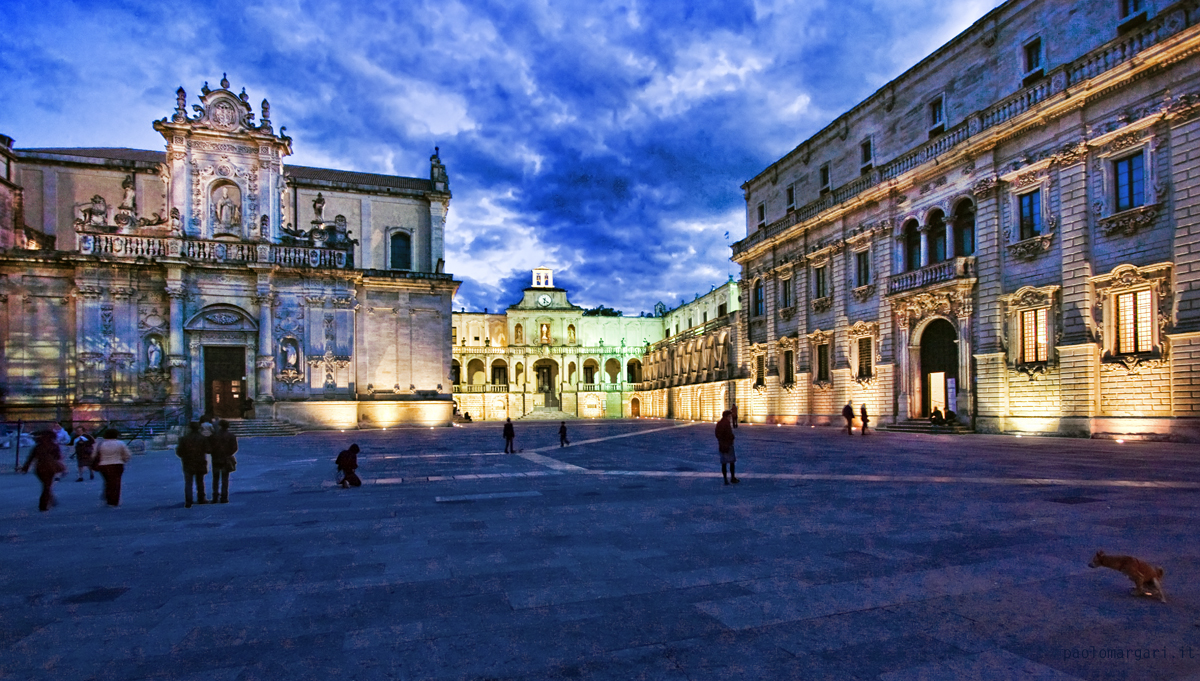
\includegraphics[height=1.05\paperheight]{Lecce1.jpg}};}
\begin{frame}
\centering
\footnotesize
\maketitle
\vspace{-.25cm}
\tiny{\textbf{Acknowledgements:} SeaDataNet, EMODnet Chemistry, \\
EMODnet Biology, STARESO}
\vspace{.125cm}

\begin{figure}
\centering

\includegraphics[width=.1\paperwidth]{gherlogo_transparent.PNG}\hspace*{.5cm}
\includegraphics[width=.1\paperwidth]{logo_ulg}\hspace*{.5cm}
\includegraphics[width=.1\paperwidth]{Logo_SeaDataNet_fond_transparent}\hspace*{.5cm}
\includegraphics[width=.07\paperwidth]{logo_emodnet}\hspace*{.5cm}
\includegraphics[width=.09\paperwidth]{Logo_Stareso}
\end{figure}

\end{frame}
}}
%-------------------------------------------------------------------------

\parindent 0cm

\author[Sylvain~Watelet, Alexander Barth, Aida Alvera-Azc\'{a}rate, Mohamed~Ouberdous, Charles~Troupin \& Jean-Marie~Beckers]{Sylvain~Watelet, Alexander Barth, Aida Alvera-Azc\'{a}rate,\\ Mohamed~Ouberdous,
 Charles~Troupin, \& Jean-Marie~Beckers}
  
\title[]{\diva Lecce 2016}
\subtitle{\diva in 2 dimensions}
\date{}
\begin{document}

\maketitlepage % defined in GHERheader2013.tex

%--------------------------------------------------------------------------------------------------------
\begin{frame}
\frametitle{Interpolation 150 years ago\ldots}

\begin{figure}[H]
\centering
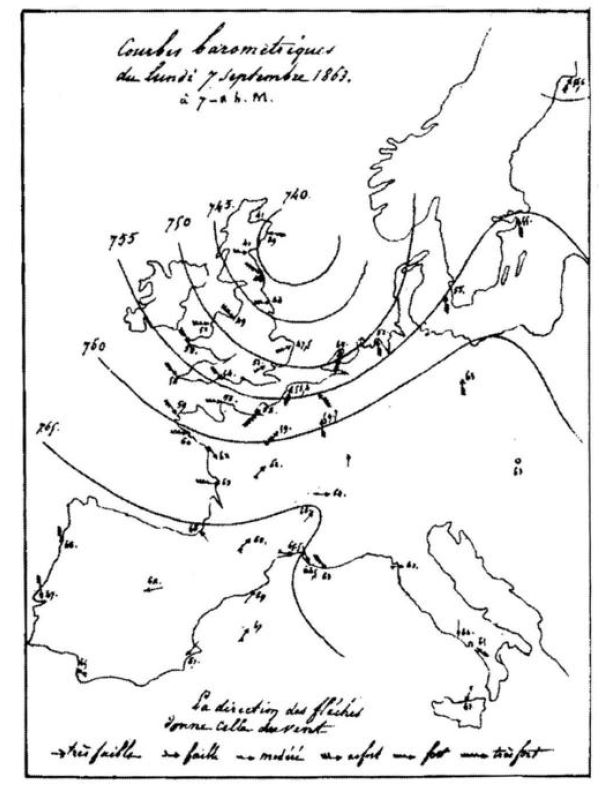
\includegraphics[width=.55\columnwidth]{oldschool_interp}
\end{figure}


\end{frame}
%--------------------------------------------------------------------------------------------------------

\begin{frame}
\frametitle{What is \diva?}

\begin{columns}[totalwidth=\textwidth]
\column{.5\textwidth}
\textbf{D}ata\\
\textbf{I}nterpolating\\
\textbf{V}ariational\\
\textbf{A}nalysis
\column{.5\textwidth}
\begin{figure}[H]
\centering

\includegraphics[width=.9\columnwidth]{Logo_diva_1500}
\end{figure}
\end{columns}

\vspace*{.5cm}

\begin{description}
\item[What is \diva?]
\begin{itemize}
\footnotesize
\item[]
\item a method to produce gridded fields
\item a set of bash scripts and Fortran programs
\item[]
\end{itemize}

\item[What is not \diva?]

\begin{itemize}
\footnotesize
\item[]
\item a plotting tool 
\item a \textit{black-box}
\item a numerical model
\end{itemize}

\end{description}
\end{frame}
%----------------------------------------------------------------------------------------------------

\begin{frame}[t]
\footnotesize
\frametitle{A little bit of history}

\begin{description}

\item<1->[Code development] (1990-1996)

\onslide*<1>{
\begin{itemize}
\scriptsize
\item Variational Inverse Method (VIM) \cita{(Brasseur, 1991, JMS, JGR)}
\item cross-validation  \cita{(Brankart and Brasseur, 1996, JAOT)}
\item error computation \cita{(Brankart and Brasseur, 1998, JMS;\\
Rixen et al., 2000, OM)}
\end{itemize}
}


\item<2->[2D-analysis] (2006-2007)

\onslide*<2>{
\begin{itemize}
\scriptsize
\item set of bash scripts  (\texttt{divamesh}, \texttt{divacalc}, \ldots)
\item Fortran executables
\item parameters optimization tools
\item Matlab/Octave scripts for plotting
\end{itemize}
}

\item<3->[3D-analysis] (2007-2008)

\onslide*<3>{
\begin{itemize}
\scriptsize
\item superposition of 2D layers
\item automated treatment and optimization
\item stability constraint \cita{(Ouberdous et al.)}
\end{itemize}
}


\item<4->[4D-analysis ] (2008-2009)

\onslide*<4>{
\begin{itemize}
\scriptsize
\item start from \textsf{ODV} spreadsheet
\item \textit{detrending} (with J.~Carstensen, DMU)
\item NetCDF 4-D climatology files
\end{itemize}
}

\item<5->[Web tools ] \hspace{1cm}

\onslide*<5>{
\begin{itemize}
\scriptsize
\item On-line analysis \cita{(Barth et al., 2010, Adv. Geosci.)}\\
\url{http://gher-diva.phys.ulg.ac.be/web-vis/diva.html}
\item Climatology viewer: \url{http://gher-diva.phys.ulg.ac.be/web-vis/clim.html}
\end{itemize}
}


\item<6->[2011-2012] \hspace{1cm}

\onslide*<6>{
\begin{itemize}
\scriptsize
\item multivariate approach
\item data transformation tools 
\item 4-D graphical interface
\item implementation of \textit{source/decay} terms
\item advanced error computation  \cita{(Troupin et al., 2012, OM)}
\end{itemize}
}

\item<7->[2013-2015] \hspace{1cm}

\onslide*<7>{
\begin{itemize}
\item Modernisation of the code structure
\item n-dimensional generalisation 
\item optimized and approximate error calculations (clever poor man)
\end{itemize}
}

\item<8->[On-going:] \hspace{1cm}

\onslide*<8>{
\begin{itemize}
\item Analysis at a specific distance from the bottom
\item Correlated observations errors (data weighting)
\item ... \Coffeecup
\end{itemize}
}

\item<9->[General:] \fbox{user-driven developments}


\end{description}		
\end{frame}

%--------------------------------------------------------------------------------------------------------
\begin{frame}
\frametitle{\diva history}

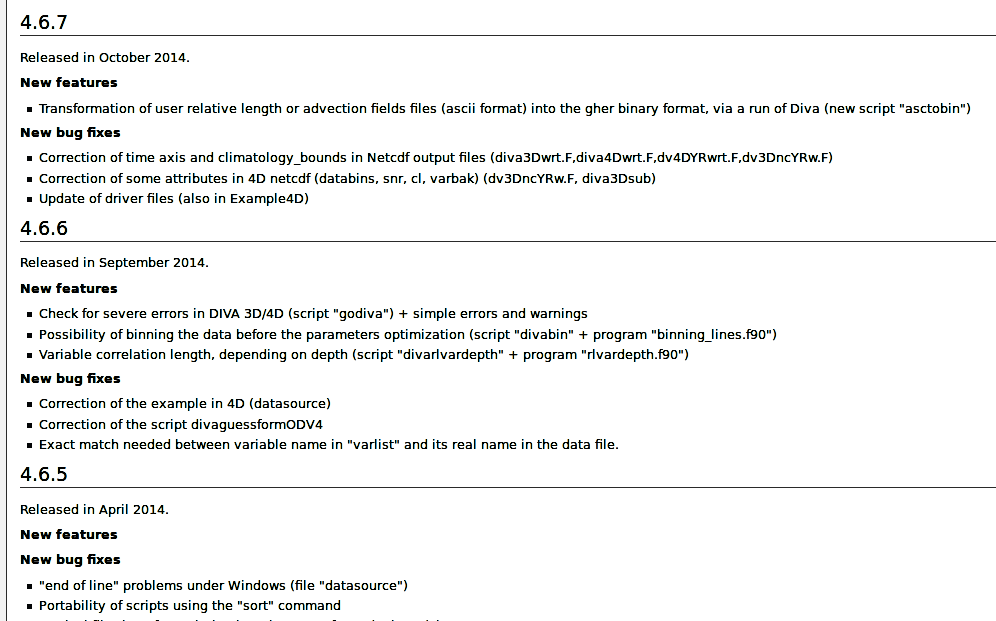
\includegraphics[width=0.9\textwidth]{diva-history}
\begin{itemize}
\item \url{http://modb.oce.ulg.ac.be/mediawiki/index.php/New_Diva_Features}
\end{itemize}
\end{frame}

%--------------------------------------------------------------------------------------------------------
\begin{frame}
\frametitle{\diva related tools}

\begin{description}
\item[\diva:] base tool (command line), 2D analysis
\item[\textsf{Godiva}:] automatic repetition of 2D analysis  
\item[\diva-on-web:] 2D analysis with your data on our server  
\item[OceanBrowser:] visualisation tool of 4D NetCDF files
\item[\textsf{divand}:] multi-dimension analysis (lon, lat, time, depth)
\item[\textsf{divaformatlab}:] wrapper to use in matlab
\item[Clone-diva-x.x.x:] virtual machine containing diva-x.x.x + other stuff (gfortran, netcdf,...)
\end{description}
\end{frame}

%---------------------------------------------------------------------

\begin{frame}
\frametitle{Common problem}
\centerline{
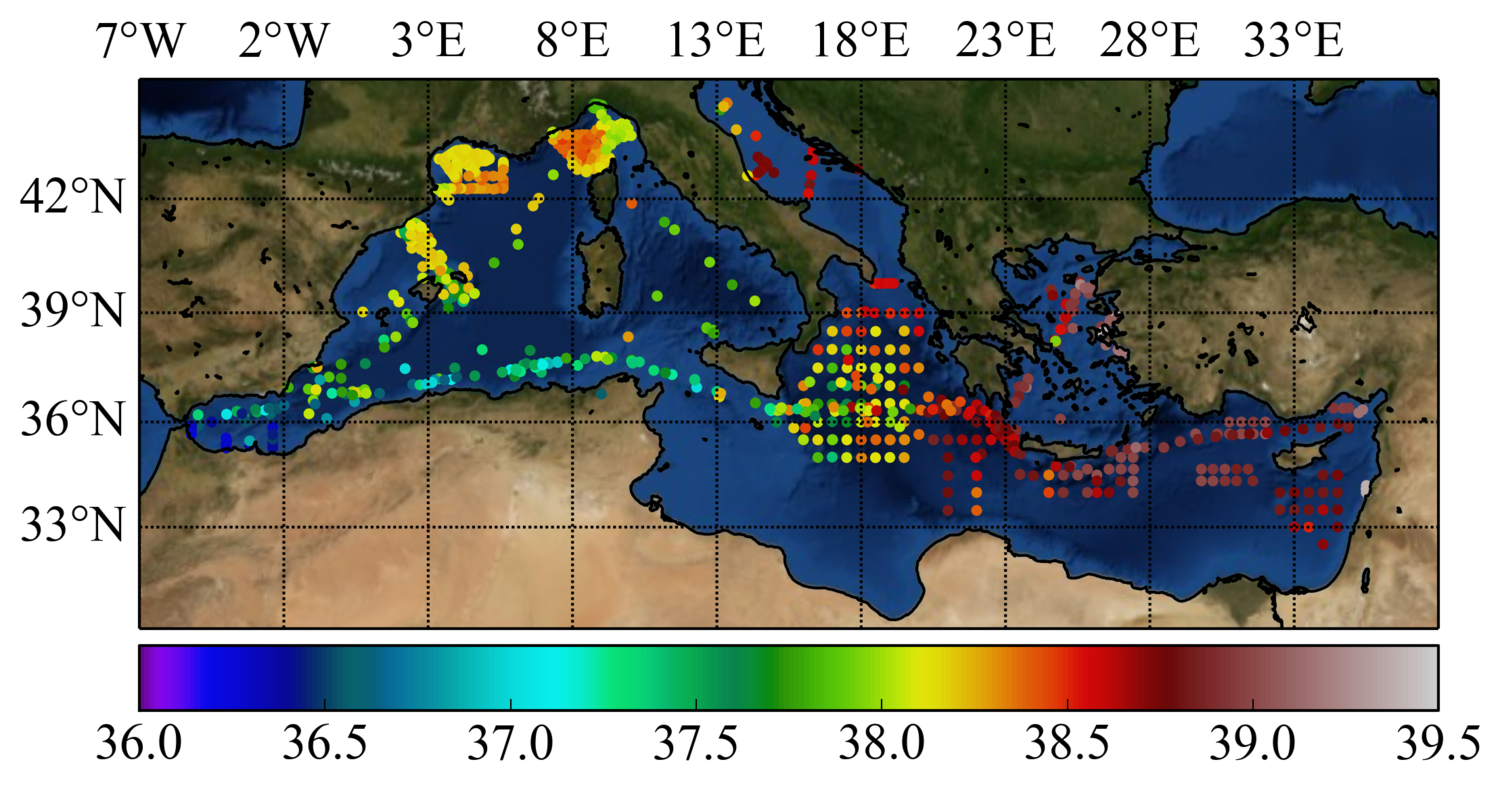
\includegraphics[width=0.75\textwidth]{medsea_data}
}
% Use divaonweb interface

Appears when
\begin{itemize}
\item trying to produce maps
\item calculate volume averages
\item prepare initial conditions for models
\item quality control of data 
\item ...
\end{itemize}
\end{frame}

%---------------------------------------------------------------------

\begin{frame}
\frametitle{The gridding problem}

Gridding is the determination of a field $\phi(\vect{r})$, on regular
grid of positions $\vect{r}$ based on arbitrarily located
observations.  Often the vector $\vect{r}$ is on a 2D, 3D or even 4D space.\\

\parbox[c]{.45\linewidth}{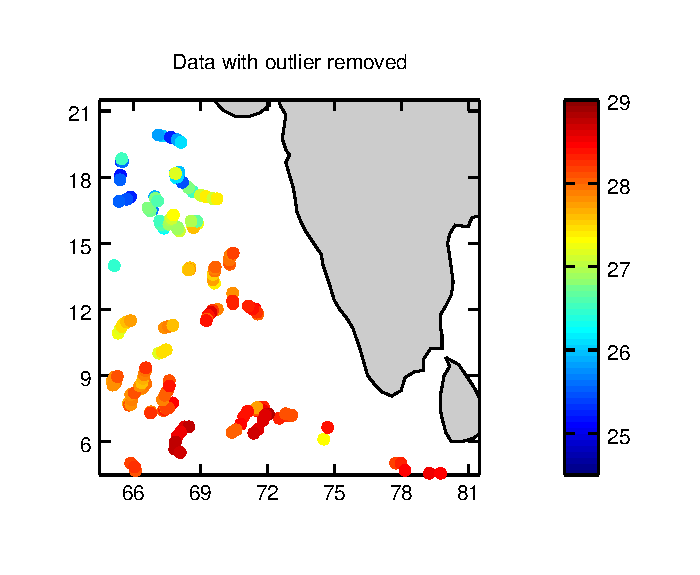
\includegraphics[width=\linewidth, trim=0 25 0 15,clip]{oi_used_data}} $\rightarrow$
\parbox[c]{.45\linewidth}{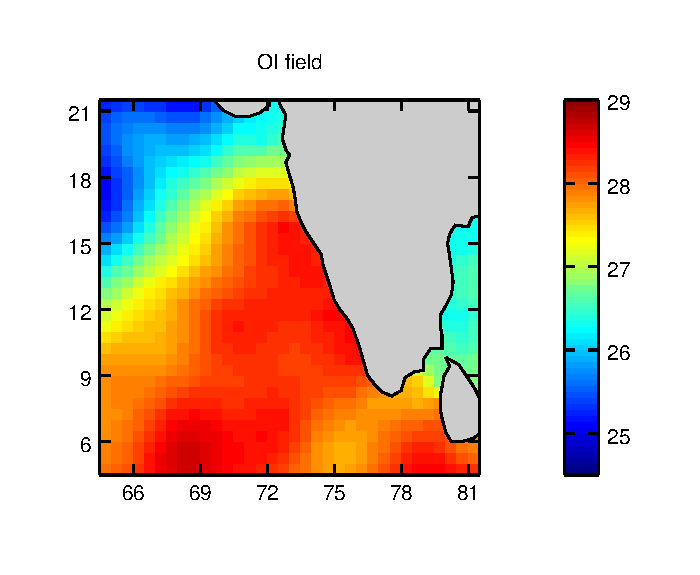
\includegraphics[width=\linewidth, trim=0 25 0 15,clip]{oi_field}}

\begin{itemize} 
\item The fewer observations are available, the harder the gridding problem is
\item In oceanography, \textit{in situ} observations are sparse
\item Observations are inhomogeneously distributed in space and time (more observations in the coastal zones and in summer)
\item The variability of the ocean is the sum of various processes
occurring at different spatial and temporal scales. 
\end{itemize}

\end{frame}

%---------------------------------------------------------------------

\begin{frame}
\frametitle{The gridding problem}

\begin{figure}[H]
\centerline{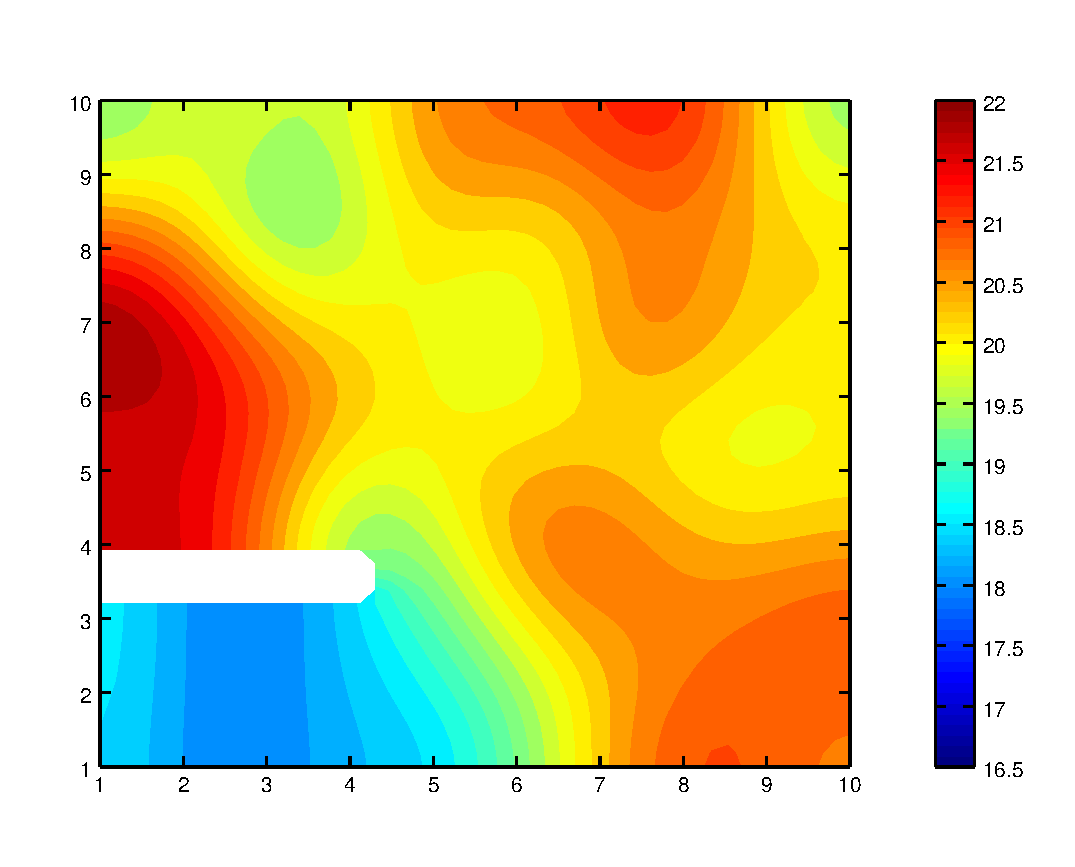
\includegraphics[width=0.5\linewidth, trim=0 28 0 37,clip]{dan_field}}
\caption{Example of oceanographic field.}
\label{dan_field}
\end{figure}

\vspace{-1cm}

\begin{itemize}
\item Figure \ref{dan_field} shows an idealized square domain with a barrier (\textit{e.g.} a peninsula or a dike).
\item  This field is the true field  that we want to reconstruct based on observations. Let's assume that the field
represents temperature. 
\item The barrier suppresses the exchanges between each side of the barrier.
\item The field varies smoothly over some length-scale
\end{itemize}

\end{frame}

%---------------------------------------------------------------------

\begin{frame}
\frametitle{Sampling locations}

\begin{figure}[H]
\centerline{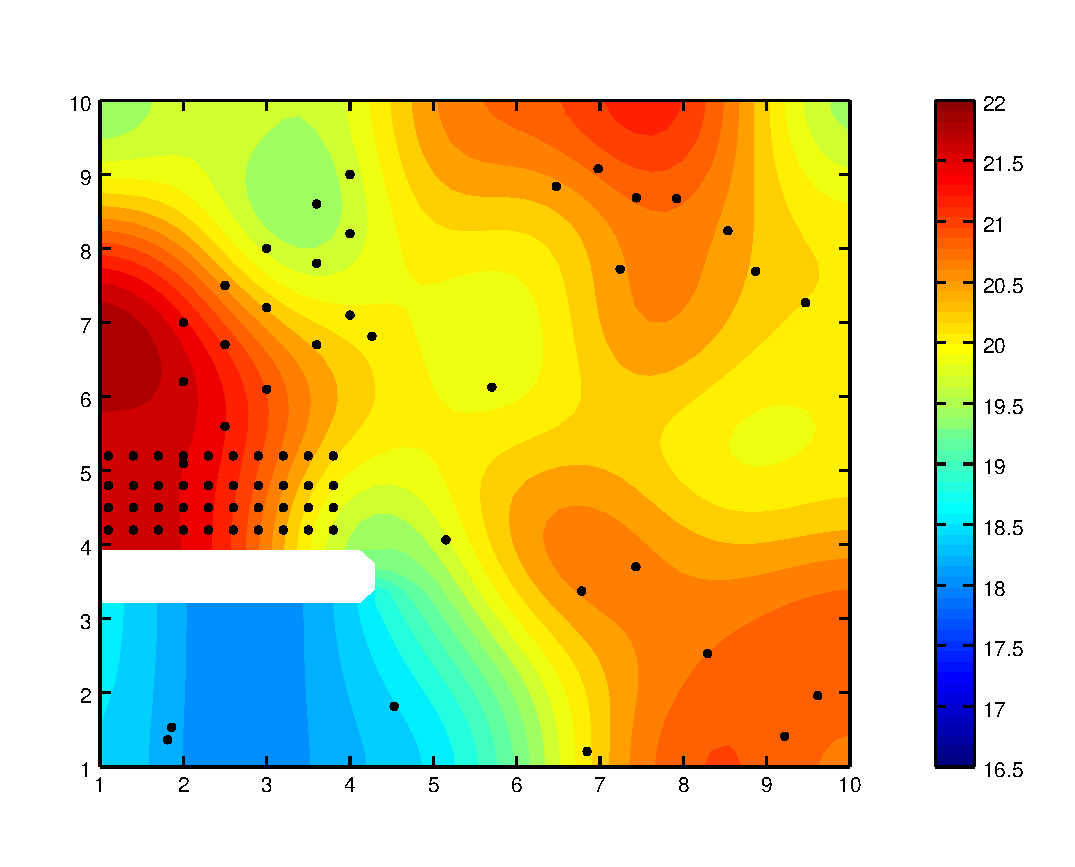
\includegraphics[width=0.5\linewidth, trim=0 28 0 37,clip]{dan_field_obs}}
\caption{Sampling locations within the domain}
\label{dan_field_obs}
\end{figure}

\vspace{-1cm}

\begin{itemize}
\item In regions where a measurement campaign has been
carried out, a higher spatial coverage is achieved. 
\item Large gaps are also present. 
\item Based on the value of the field at the shown location,
we will estimate the true field.
\end{itemize}

\end{frame}

%---------------------------------------------------------------------

\begin{frame}
\frametitle{True field at the sampling locations}

\begin{figure}[H] 
\centerline{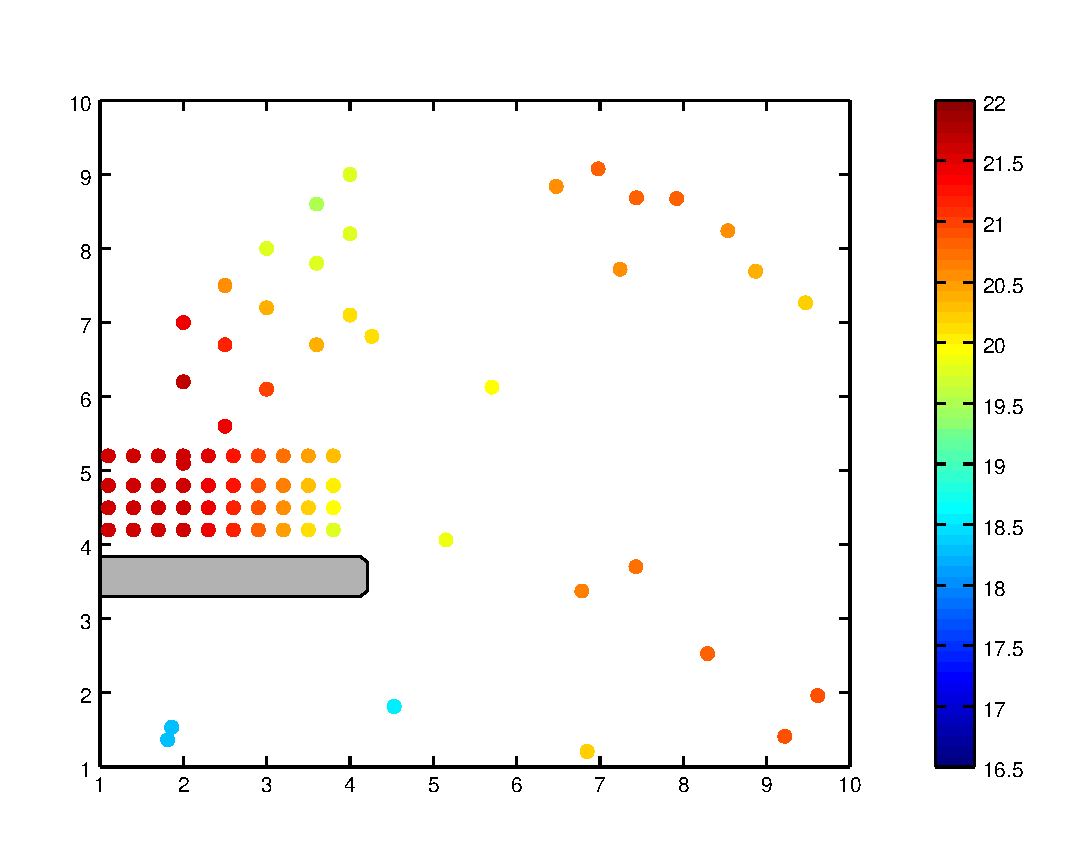
\includegraphics[width=0.5\linewidth, trim=0 28 0 37,clip]{dan_obs}}
\caption{Value of the true field extract at the location of the
  observations.}
\label{dan_obs}
\end{figure}

\vspace{-1cm}

\begin{itemize} 
\item only the value of the observations is shown
\item  some information about the position of the
structures and fronts is lost 
\item no method can provide exactly the true field.
\item the
more information about its structure and evolution we include in the
analysis, to close we can get to the true field.
\end{itemize}

\end{frame}

%---------------------------------------------------------------------

\begin{frame}
\frametitle{Observation errors}

Observations are in general affected by different error sources and
other ``problems'' that need to be taken into account:

\begin{enumerate}
\item Instrumental errors (limited precision or possible bias of the
  sensor)
\item Representative errors: the observations do not necessarily
  corresponds to the field we want to obtain. For example, we want to
  have a monthly average, but the observations are instantaneous (or
  averages over a very short period of time).
\item Synopticity errors: all observations are not taken at the same time.
\item Other errors sources: human errors (e.g. permutation of
  longitude and latitude), transmission errors, malfunctioning of the
  instrument, wrong decimal separators...
\end{enumerate}

Quality control is an important step to exclude suspicious data from
the analysis. But since this is a subjective decision, the data should
never be deleted but flagged as suspicious or bad data.

\end{frame}

%---------------------------------------------------------------------

\begin{frame}
\frametitle{Observation errors}

\begin{figure}[H] 
\centerline{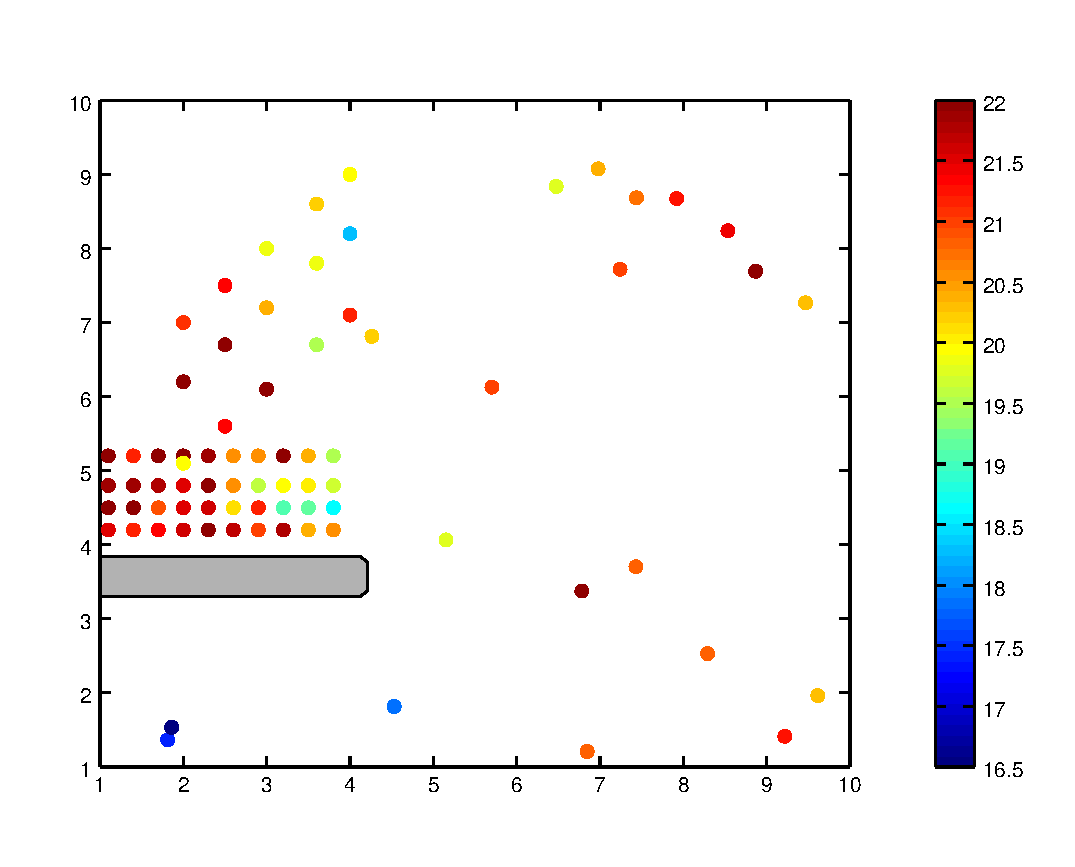
\includegraphics[width=0.5\linewidth, trim=0 28 0 37,clip]{dan_obs_err}}
\caption{Observation with errors}
\label{dan_obs_err}
\end{figure}

\vspace{-1cm}

In figure \ref{dan_obs_err}, a random perturbation was added to the
observation shown in figure \ref{dan_obs}. This simulates the impact
of the different error sources. To simplify matters, each observation
was perturbed independently.\\

\end{frame}

%---------------------------------------------------------------------

\begin{frame}
\frametitle{Solutions - Subjective methods}

\centerline{
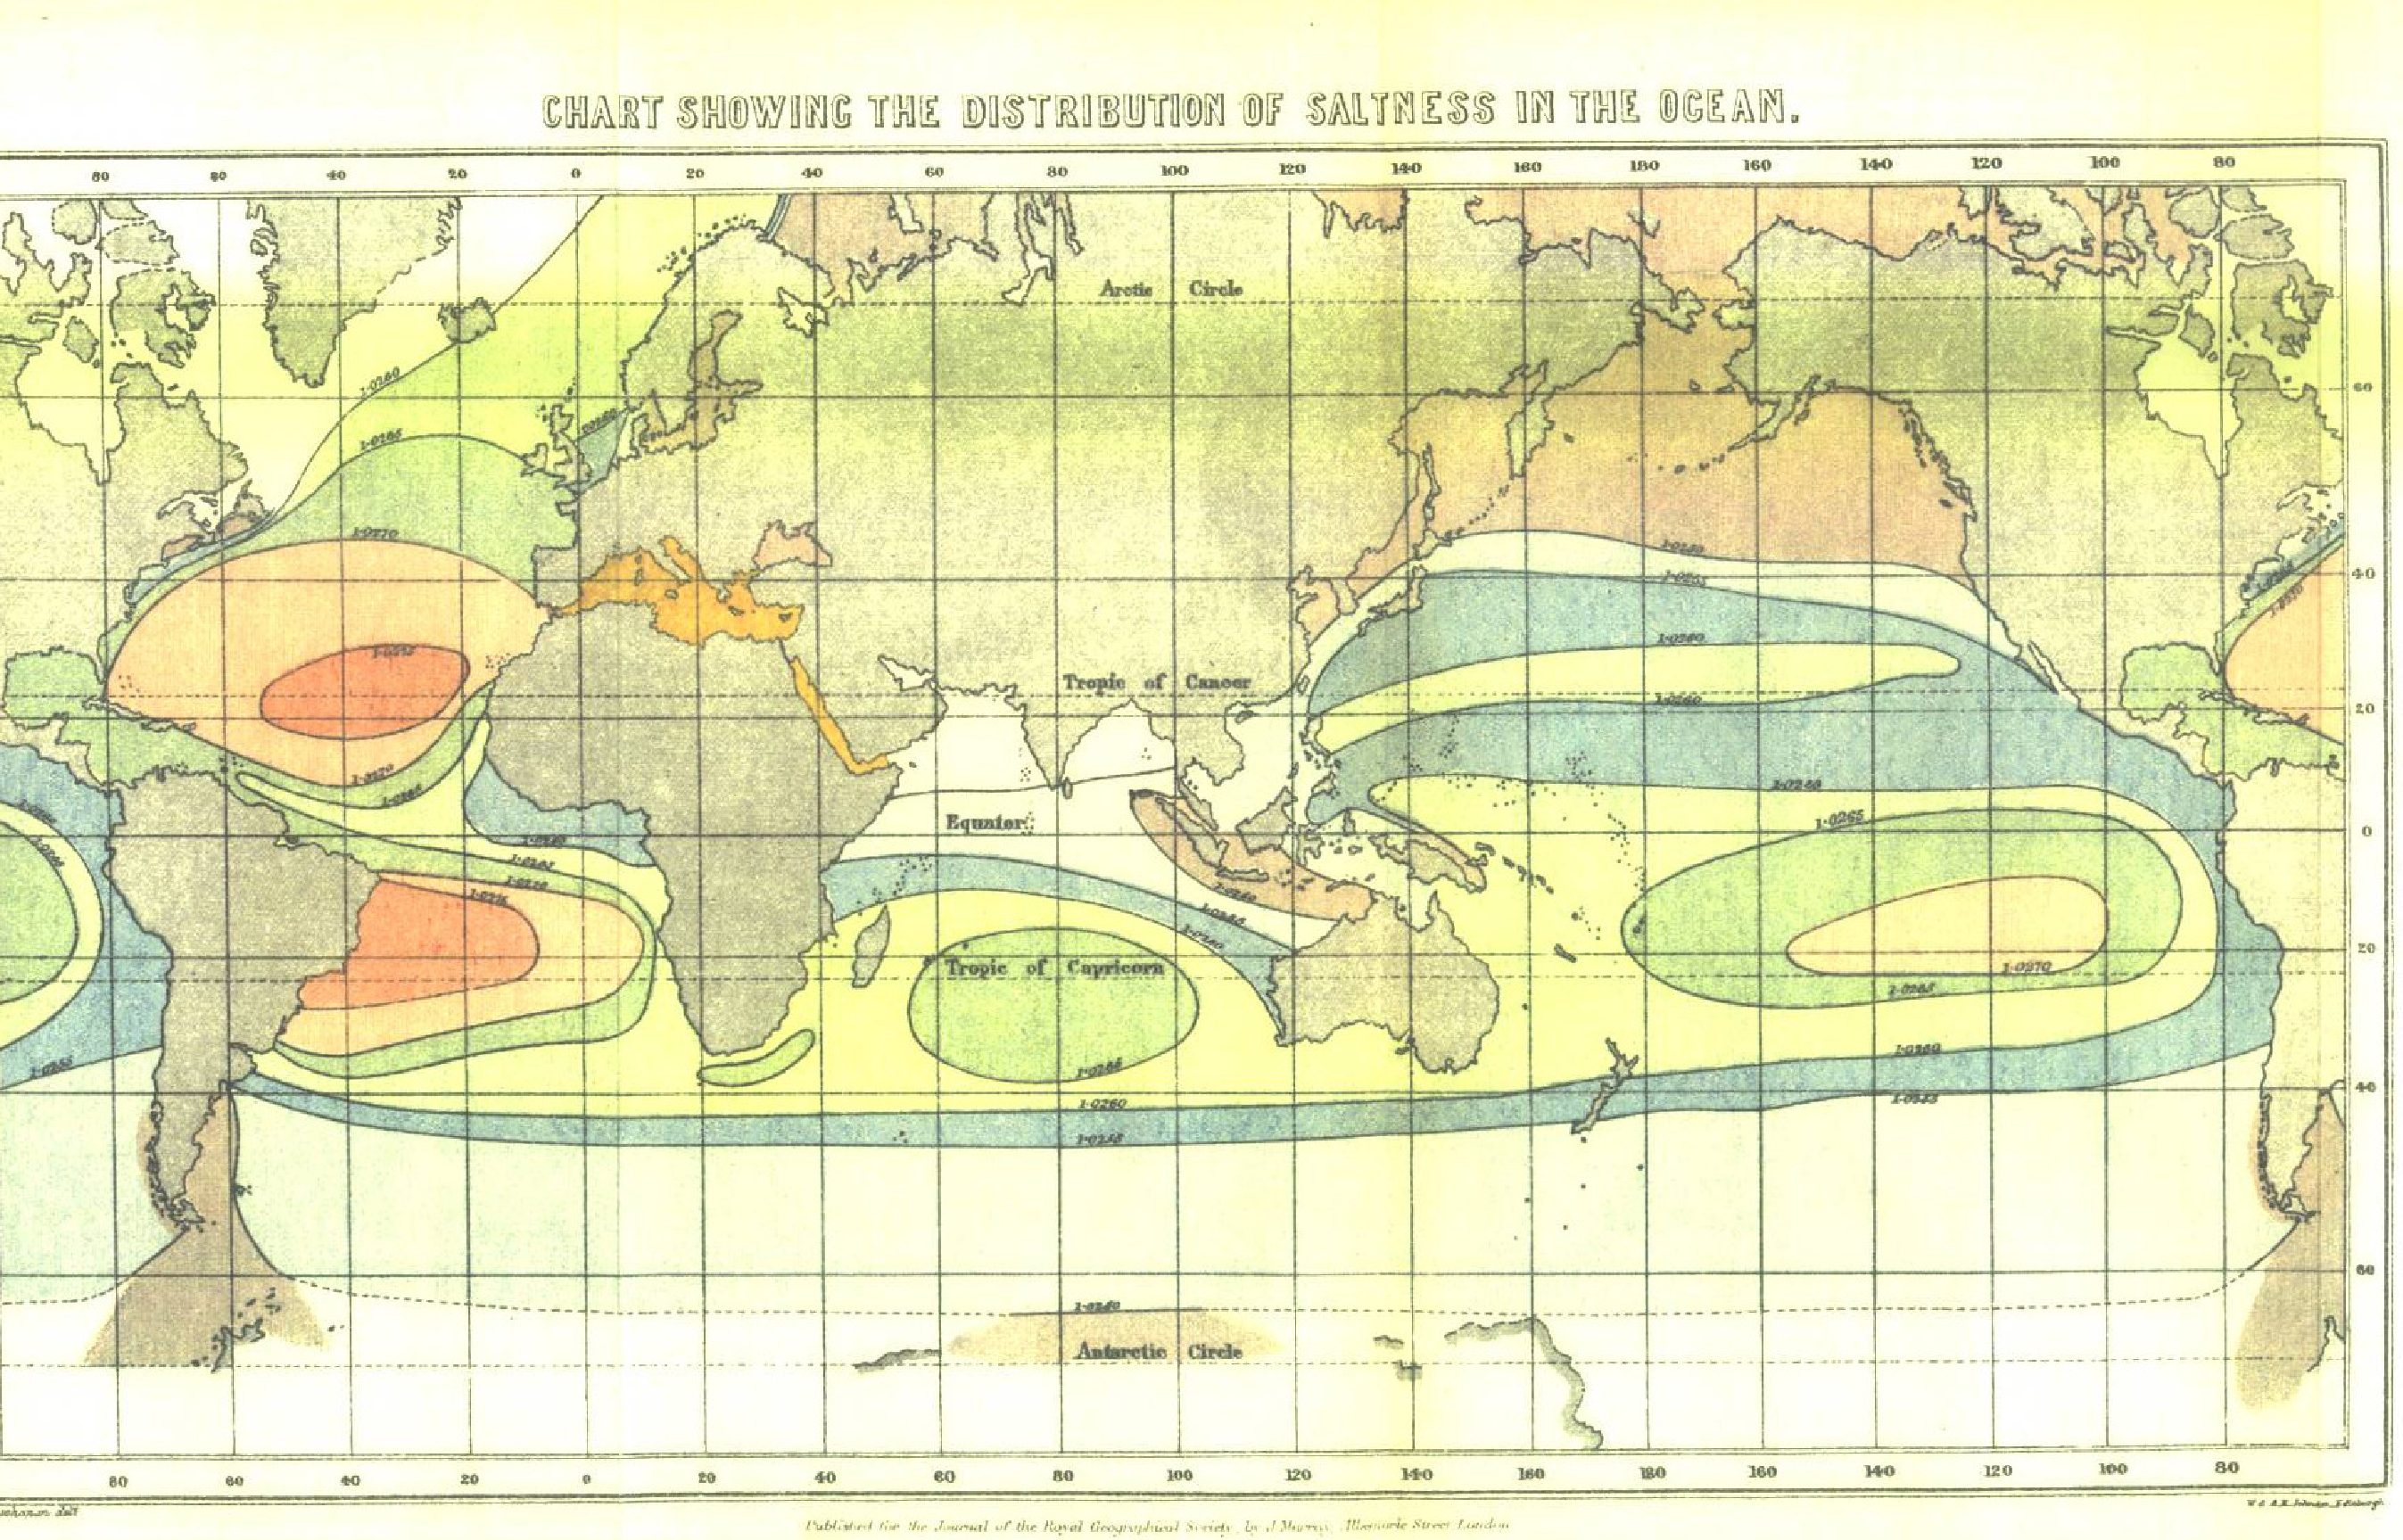
\includegraphics[width=0.9\textwidth]{discovery}
}
\end{frame}

%---------------------------------------------------------------------

\begin{frame}
\frametitle{Solutions - Subjective methods}

\begin{figure}[H]
\centerline{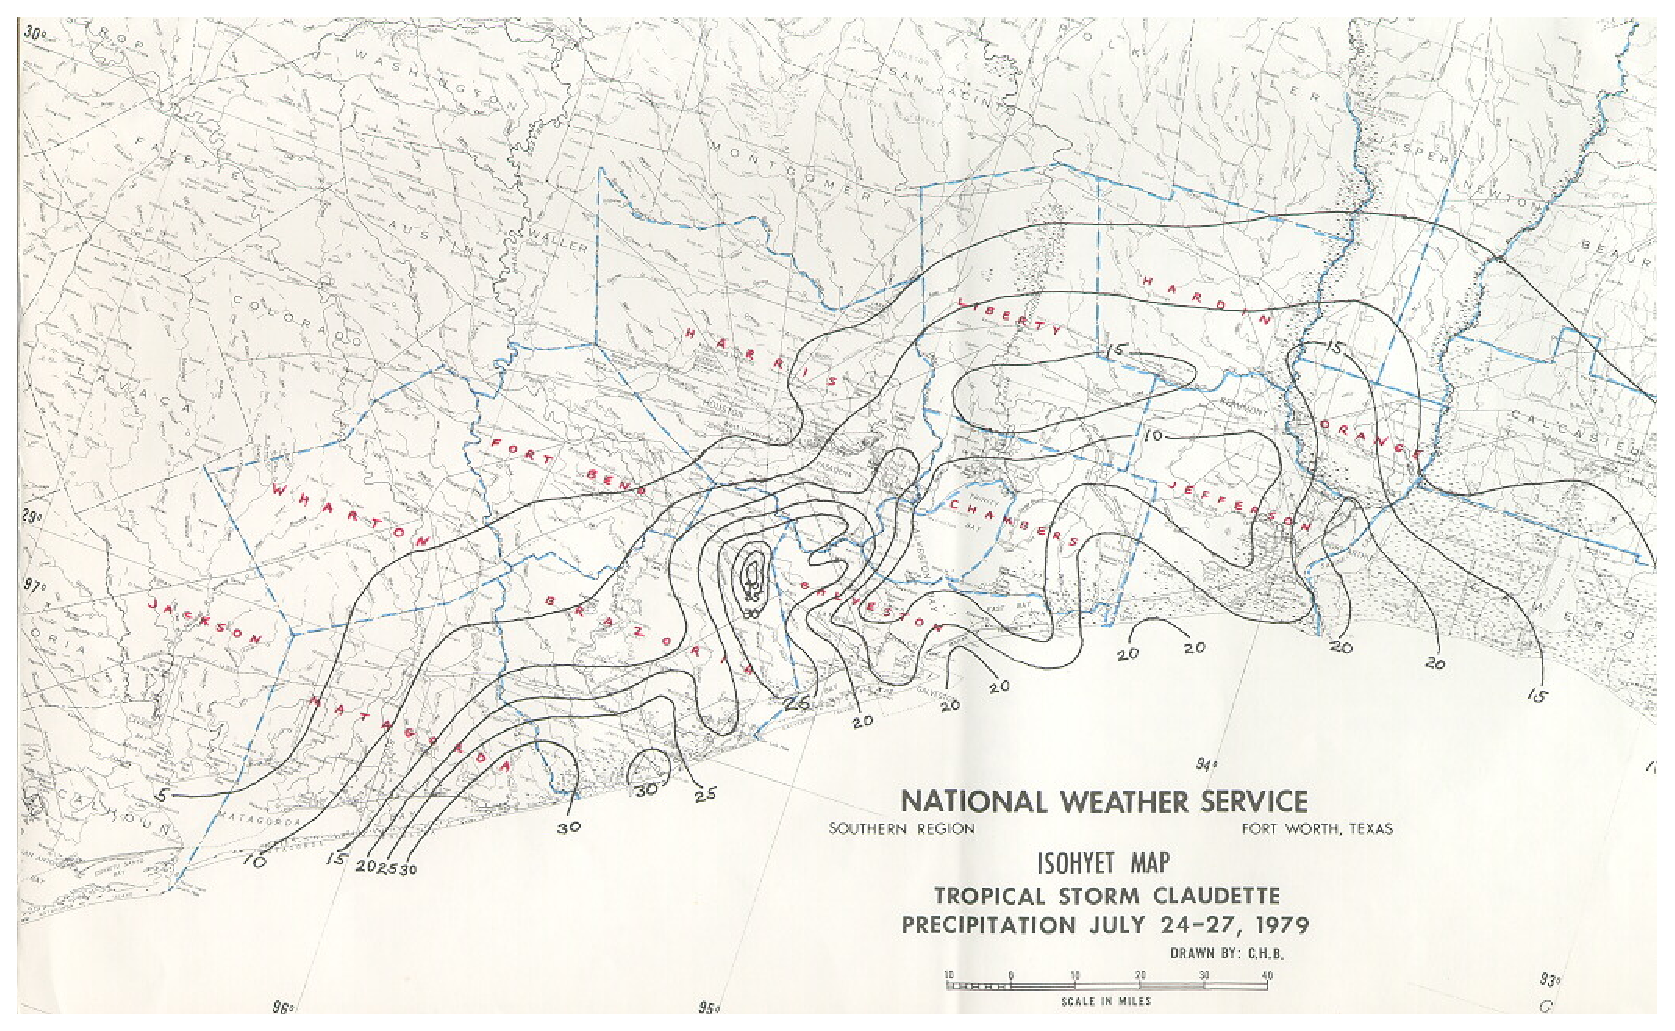
\includegraphics[width=\linewidth]{tropical_storm_claudette}}
\caption{Isohyet (lines of constant precipitation) drawn by hand (from \url{http://www.srh.noaa.gov/hgx/hurricanes/1970s.htm})}
\label{fig:byhand}
\end{figure}

\end{frame}

%---------------------------------------------------------------------

\begin{frame}
\frametitle{Interpolation or Analysis ?}

Because observations have errors, it is always better to produce a
field approximation and never a strict interpolation. 

\begin{figure}[H]
\centerline{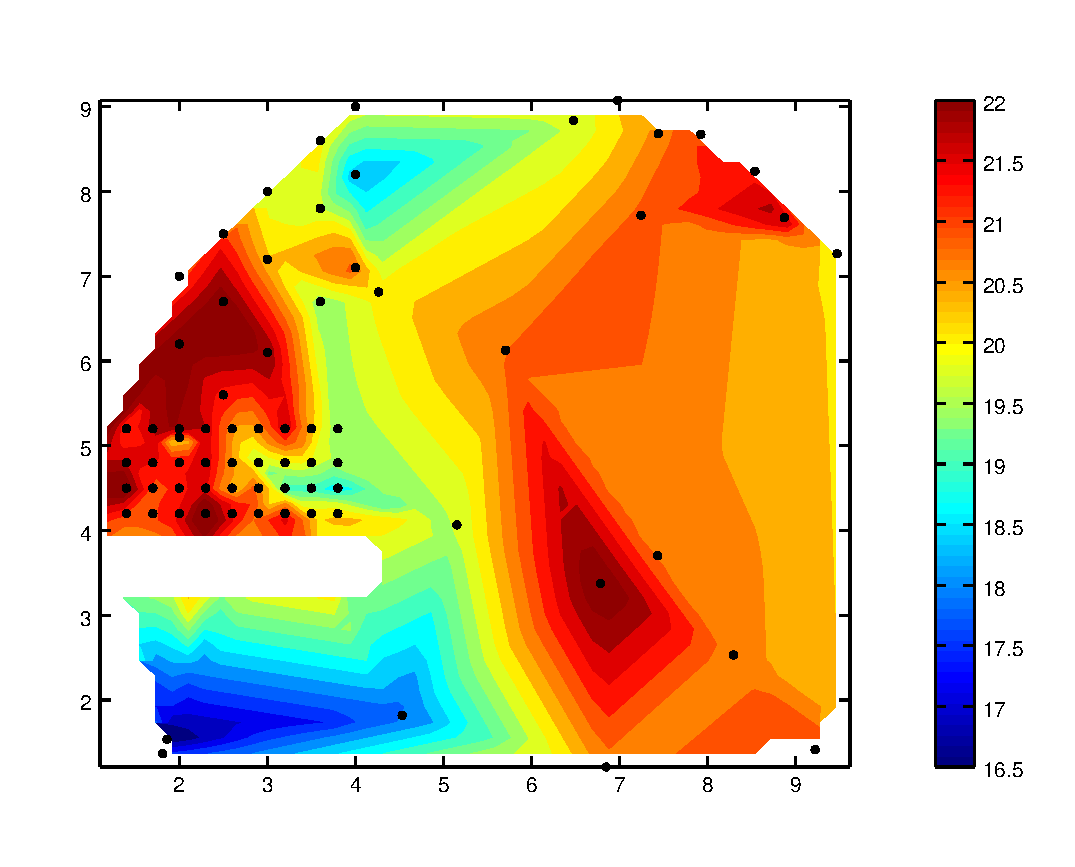
\includegraphics[width=0.5\linewidth, trim=0 28 0 37,clip]{dan_griddata}}
\caption{Gridded field using linear interpolation. This method is
  implemented in the function \texttt{griddata} of Matlab and GNU
  Octave.}
\label{dan_griddata}
\end{figure}

\vspace{-1cm}

{\fontsize{9pt}{10}\selectfont
\begin{itemize}
\item Figure
\ref{dan_griddata} shows what would happen if the observations would
have been interpolated linearly. 
\item The domain is
  decomposed into triangles where the vertices are the location of the
  data points based on the Delaunay triangulation. 
\item Within each
  triangle, the value is interpolated linearly. 
%\item The noise on the observations is in
%general amplified when higher order schemes, such as cubic
%interpolation, are used.
\end{itemize}
}

\end{frame}

%---------------------------------------------------------------------

\begin{frame}
\frametitle{Solutions - Objective methods}

\begin{itemize}
\item Subjective method is not sufficiently ... objective.
\item Data Assimilation: region and model dependent.
\end{itemize}
$\Rightarrow$ Objective analysis of data that are anomalies with
respect to a background field $\varphi_b(\vect{r})$.

As opposed to the subjective method, objective analysis techniques aim
to use mathematical formulations to infer the value of the field at
unobserved locations based on the observation $d_j$.  Most objective
methods can be expressed as a linear combination of data anomalies
$d_j$ using weights $w_j$:
\vspace{-0.5cm}
\begin{equation}
\varphi(\vect{r}) = \varphi_b(\vect{r}) ~+~ \sum_{j=1}^{N_d} w_j d_j
\end{equation}

The field $\varphi(\vect{r})$ can be evaluated in any position
$\vect{r}$, hence gridding is possible.  The {\color{red}background field (or
first guess)} $\varphi_b$ is defined {\it a priori} and anomalies
calculated with respect to this reference field (for example a
climatological average).  There are several ways to define the
weighting function $w_j$, which result in different gridding
techniques. %We will review in the following the most used gridding
%methods.

\end{frame}

%---------------------------------------------------------------------

\begin{frame}
\frametitle{Cressman method}

Cressman weights depend only on the distance $r$ between the location
$\vect{r}$ where the value of the field should be estimated and the
location of the observation $\vect{r}_j$:

\begin{equation}
r = {\left|\vect{r}-\vect{r}_j\right|}
\end{equation}

The weights are then parameterized according to,

\begin{equation}
\begin{array}{rclrr}
\tilde{w}(r) &=& \frac{R^2-r^2}{R^2+r^2} & \mbox{for} & r < R \\ &=& 0
& \mbox{for} & r \ge R
   \end{array}
\end{equation}

The weights as a function of distance are shown in figure
\ref{fig:dan_cressman_w}.  Weights must be scaled by their sum to
ensure no bias.

\begin{equation}
w_j= \tilde{w}_j/\sum_j \tilde{w}_j
\end{equation}

\end{frame}

%---------------------------------------------------------------------

\begin{frame}
\frametitle{Cressman method}

\begin{figure}[H] 
\centerline{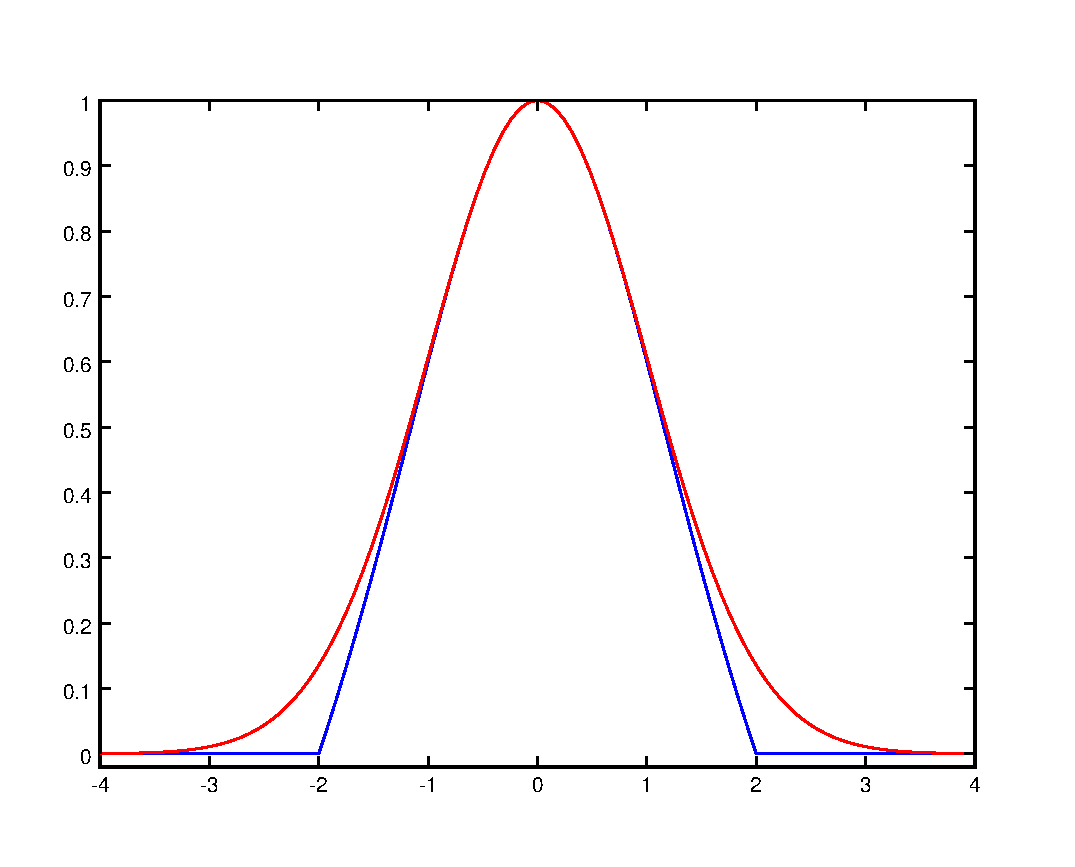
\includegraphics[width=0.5\linewidth, trim=0 28 0 37,clip]{dan_cressman_w}}
\caption{Cressman weights for $R=2$ (blue) and Barnes weights for
  $R=1$ (red).}
\label{fig:dan_cressman_w}
\end{figure}

\vspace{-1cm}

The search radius $R$ is the typical control parameter and defines the
length-scale over which an observation is used.  This length scale
can be made to vary in space depending on data coverage and/or
physical scales. This parameter is chosen by the users based on their
knowledge of the domain and the problem.

\end{frame}

%---------------------------------------------------------------------

\begin{frame}
\frametitle{Cressman method}

\begin{figure}[H]
\centerline{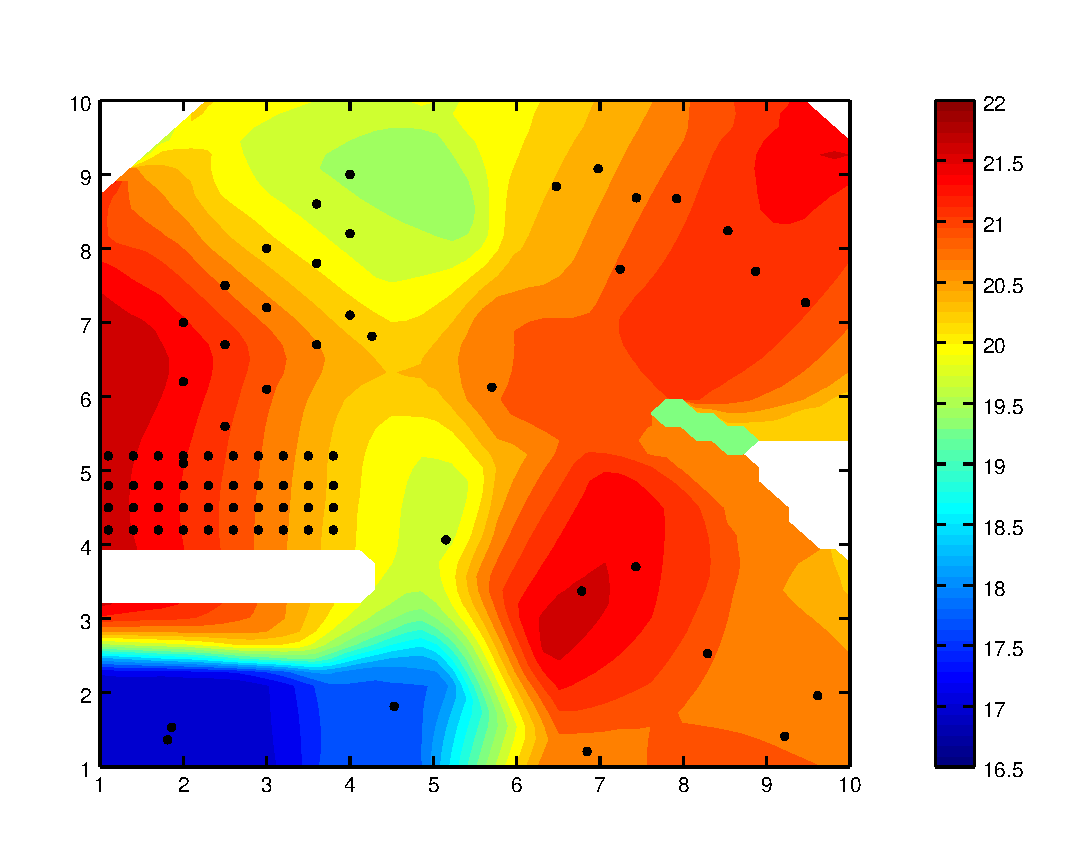
\includegraphics[width=0.5\linewidth, trim=0 28 0 37,clip]{dan_cressman}}
\caption{Gridded field by Cressman weighting}
\label{fig:dan_cressman}
\end{figure}

\vspace{-1cm}

{\fontsize{9pt}{10}\selectfont The Cressman weighting is a very simple and numerically quite
efficient method. However, it suffers from some limitations which are
apparent in figure \ref{fig:dan_cressman}.

\begin{itemize}
\item No estimate can be obtained at locations when no observation is
  located within the $R$.
\item In regions with very few observations, the method can return a
  discontinuous field.
\item The presence of barriers
  cannot be taken into account easily.
\item All observations are assumed to have a similar error
  variance since the weighting is based only on distance.
\end{itemize}}

\end{frame}

%---------------------------------------------------------------------

\begin{frame}
\frametitle{Barnes method}

{\fontsize{9pt}{10}\selectfont As a variant of the Cressman weights, other weighting functions can be
defined. In the Barnes scheme, the weights are defined using a
Gaussian function:}

\begin{eqnarray}
\tilde{w}(d) &=& e^{-\frac{d^2}{2 R^2}}
\end{eqnarray}

\begin{figure}[H]
\centerline{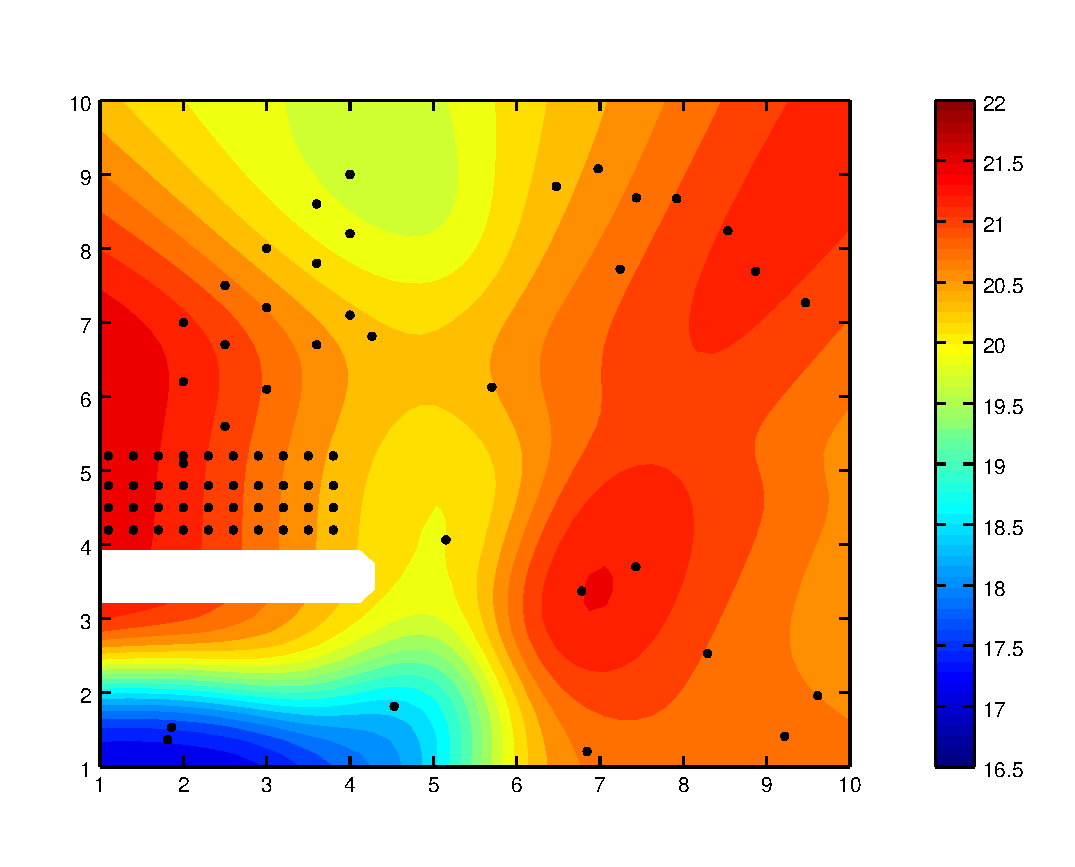
\includegraphics[width=0.5\linewidth, trim=0 28 0 37,clip]{dan_barnes}}
\caption{Gridded field using Barnes weights}
\label{dan_barnes}
\end{figure}

\vspace{-1cm}

{\fontsize{9pt}{10}\selectfont Since the Barnes weights are never zero, in principle all observations
are used for the gridding. An estimation can be obtained everywhere
(which can be accurate or not). Artificial discontinuities are avoided
using the Barnes weights (figure \ref{dan_barnes}).}

\end{frame}

%---------------------------------------------------------------------

\begin{frame}{Estimation}
\begin{itemize}
\item
Observer 1: 14$^\circ$
\item
Observer 2: 16$^\circ$
\end{itemize}

\centerline{Your best guess ?}

\only<2->{\centerline{15$^\circ$}}
\only<3>{But what if observer 1 uses digital thermometer and observer 2 his finger ?}
\only<4>{But what if observer 1 uses digital thermometer and observer 2 his finger ?
\centerline{Best guess probably near 14$^\circ$.}}
\only<5>{But what if observer 1 uses digital thermometer and observer 2 his finger ?
\centerline{Best guess probably near 14$^\circ$.}
\begin{center}
\shabox{
Exploit knowledge of errors !}
\end{center}
}
\end{frame}

%---------------------------------------------------------------------

\begin{frame}{Optimal estimate}
\begin{equation}
T_1 = \true{T}+\epsilon_1, \quad \statmean{\epsilon_1} = 0, \quad T_2 = \true{T}+\epsilon_2, \quad \statmean{\epsilon_2} = 0
\end{equation}
statistical average, denoted by $\statmean{\quad}$ with unbiased estimates $\statmean{\epsilon_*}=0$

Linear estimate
\begin{equation}
{T}=w_1 \, T_1 ~+~ w_2 \, T_2 ~=~ (w_1+w_2) \true{T} ~+~ (w_1 \epsilon_1 + w_2 \epsilon_2)
\end{equation}
\begin{equation}
\statmean{{T}} = (w_1+w_2) \true{T},
\end{equation}
we obtain an unbiased estimate of the true state if we take $w_1+w_2=1$. This leaves one parameter free to chose: $w_2$
\begin{center}
\shabox{Exploit knowledge on errors to find optimal value of $w_2$}
\end{center}
\end{frame}

%---------------------------------------------------------------------

\begin{frame}{Choice of weighting ?}
\begin{equation}
\analyzed{T} = (1-w_2) T_1 + w_2 T_2  ~=~ T_1 + w_2 (T_2-T_1)
\end{equation}
while in reality there is an error
\begin{equation}
\analyzed{T} - \true{T} = (1-w_2) \epsilon_1 + w_2 \epsilon_2,
\end{equation}
This error is zero on average but its variance is not zero:
\begin{equation}
\statmean{(\analyzed{T}-\true{T})^2} = (1-w_2)^2 \statmean{\epsilon_1^2} + w_2^2 \statmean{\epsilon_2^2} + 2 (1-w_2) w_2 
\statmean{\epsilon_1 \epsilon_2}
\end{equation}
The actual errors $\epsilon_1$ and $\epsilon_2$ are not known, but the error variance $\statmean{\epsilon_1^2}$ are.
Often we can reasonably suppose that the errors
$\epsilon_1$ and $\epsilon_2$ are uncorrelated $\statmean{\epsilon_1 \epsilon_2}=0$. 
The error variance $\statmean{\epsilon^2}$ of the analysis is
\begin{equation}
\statmean{\epsilon^2}=(1-w_2)^2 \statmean{\epsilon_1^2} + w_2^2 \statmean{\epsilon_2^2}.
\label{eq:epsilonerror}
\end{equation}
So what ?
\end{frame}

%---------------------------------------------------------------------

\begin{frame}{Minimisation}
\begin{equation}
\statmean{\epsilon^2}=(1-w_2)^2 \statmean{\epsilon_1^2} + w_2^2 \statmean{\epsilon_2^2}.
\label{eq:epsilonerror}
\end{equation}
Naturally, the best estimate for $T$ is the one with the lowest expected error variance and we will use $w_2$, which minimizes
the right-hand side:
\begin{equation}
w_2 = \frac{\statmean{\epsilon_1^2}}{\statmean{\epsilon_1^2}+\statmean{\epsilon_2^2}}
\label{eq:weighterror}
\end{equation}
%\begin{equation}
%\analyzed{T}=   {\statmean{\epsilon_1^2} \statmean{\epsilon_2^2} \over \statmean{\epsilon_1^2} 
%+ \statmean{\epsilon_2^2} }\left( {T_1 \over \statmean{\epsilon_1^2}} + {T_2 \over \statmean{\epsilon_2^2}}\right) .
% \label{eq:analyzedTb}
%\end{equation}
\end{frame}

%---------------------------------------------------------------------

\begin{frame}{Best estimate}
With \eqref{eq:weighterror} we obtain the minimal error variance
\begin{equation}
\statmean{\epsilon^2}= {\statmean{\epsilon_1^2} \statmean{\epsilon_2^2} \over \statmean{\epsilon_1^2} 
+ \statmean{\epsilon_2^2} } = \left( 1 - {\statmean{\epsilon_1^2} \over \statmean{\epsilon_1^2} 
+ \statmean{\epsilon_2^2} } \right) \statmean{\epsilon_1^2},
\label{eq:optimalerror}
\end{equation}
while the estimate of the temperature itself reads
\begin{equation}
\analyzed{T}= T_1 ~+~ \left( {\statmean{\epsilon_1^2} \over \statmean{\epsilon_1^2} 
+ \statmean{\epsilon_2^2} } \right) \left( T_2-T_1\right).
 \label{eq:analyzedT}
\end{equation}
\begin{center}
\shabox{Error variance on the combination of $T_1$ and $T_2$ 
is smaller than both $\statmean{\epsilon_1^2}$ and $\statmean{\epsilon_2^2}$. }
\end{center}
\end{frame}

%---------------------------------------------------------------------

\begin{frame}[allowframebreaks]{Optimal Interpolation}
Same problem but data distributed in space and {\it a priori} information on background (with variance $\sigma^2$). 

Weighting of background (zero value when working with anomalies and $\sigma^2$ local variance and covariances between points) information and data points (observed values and observational error variance) 

\begin{itemize}
\item
"Model forecast": Background field.
\item
Need for  covariance of the background field between data points: each element $i,j$ of $\matr{B}$ provides the covariance between points in location $i$ and $j$. Covariance between a given point and all data points is stored in column vector $\matr{c}$ and the local variance at the analysis point is noted $\sigma^2$.
\item
Analysis $\phi$ of anomaly $\observation$ with respect to background leads to spatial analysis at any desired location of covariance between any two points is known.
\end{itemize}

\begin{equation}
\phi= {\matr{c}}^t \inv{\left( \matr{B} + \Rerr \right)} 
\observation
\label{eq:analyzedfield}
\end{equation}
with a local error variance of the analysis
\begin{equation}
\epsilon_a^2=\sigma^2 - {\matr{c}}^t \inv{\left( \matr{B} + \Rerr \right)} \matr{c}
\end{equation}
Note that inversion of matrix is needed (cost increases as the cube of number of data points).

\end{frame}

%---------------------------------------------------------------------

\begin{frame}{Background covariance}
Problem, how to specify background covariances (between all data points and between data points and the desired analysis location).
\begin{itemize}
\item $c_i$= {covariance between location of the analysis and data location of point i} = $C(x,x_i)$
\item $B_{ij}$={covariance between location of data point i and  location of point j}= $C(x_i,x_j)$
\end{itemize}
Approaches
\begin{itemize}
\item
Normally obtained via statistics on data. Seldom possible (noticable exception: satellite images).
\item
Standard OI: via functions $B_{ij}= f(r/L)$ where $r$ is the distance between points $i$ and $j$, but still function $f$ needs to be determined. $L$ is the so-called correlation length. Here statistics on all data couples as a function of distance.
Example: $f=\sigma^2 \exp(-r^2/L^2)$.
\item Via functionals (see Kernel of DIVA later)
\end{itemize}
\end{frame}

%---------------------------------------------------------------------
\begin{frame}[t]
\frametitle{DIVA: Data-Interpolating Variational Analysis}
\footnotesize

\begin{figure}[H]
\textcolor{blue}{$N_{d}$ data points $d_{i}$ $\bullet$}\quad $\rightarrow$ \quad{\textcolor{gray}{gridded field}}\\
\centering
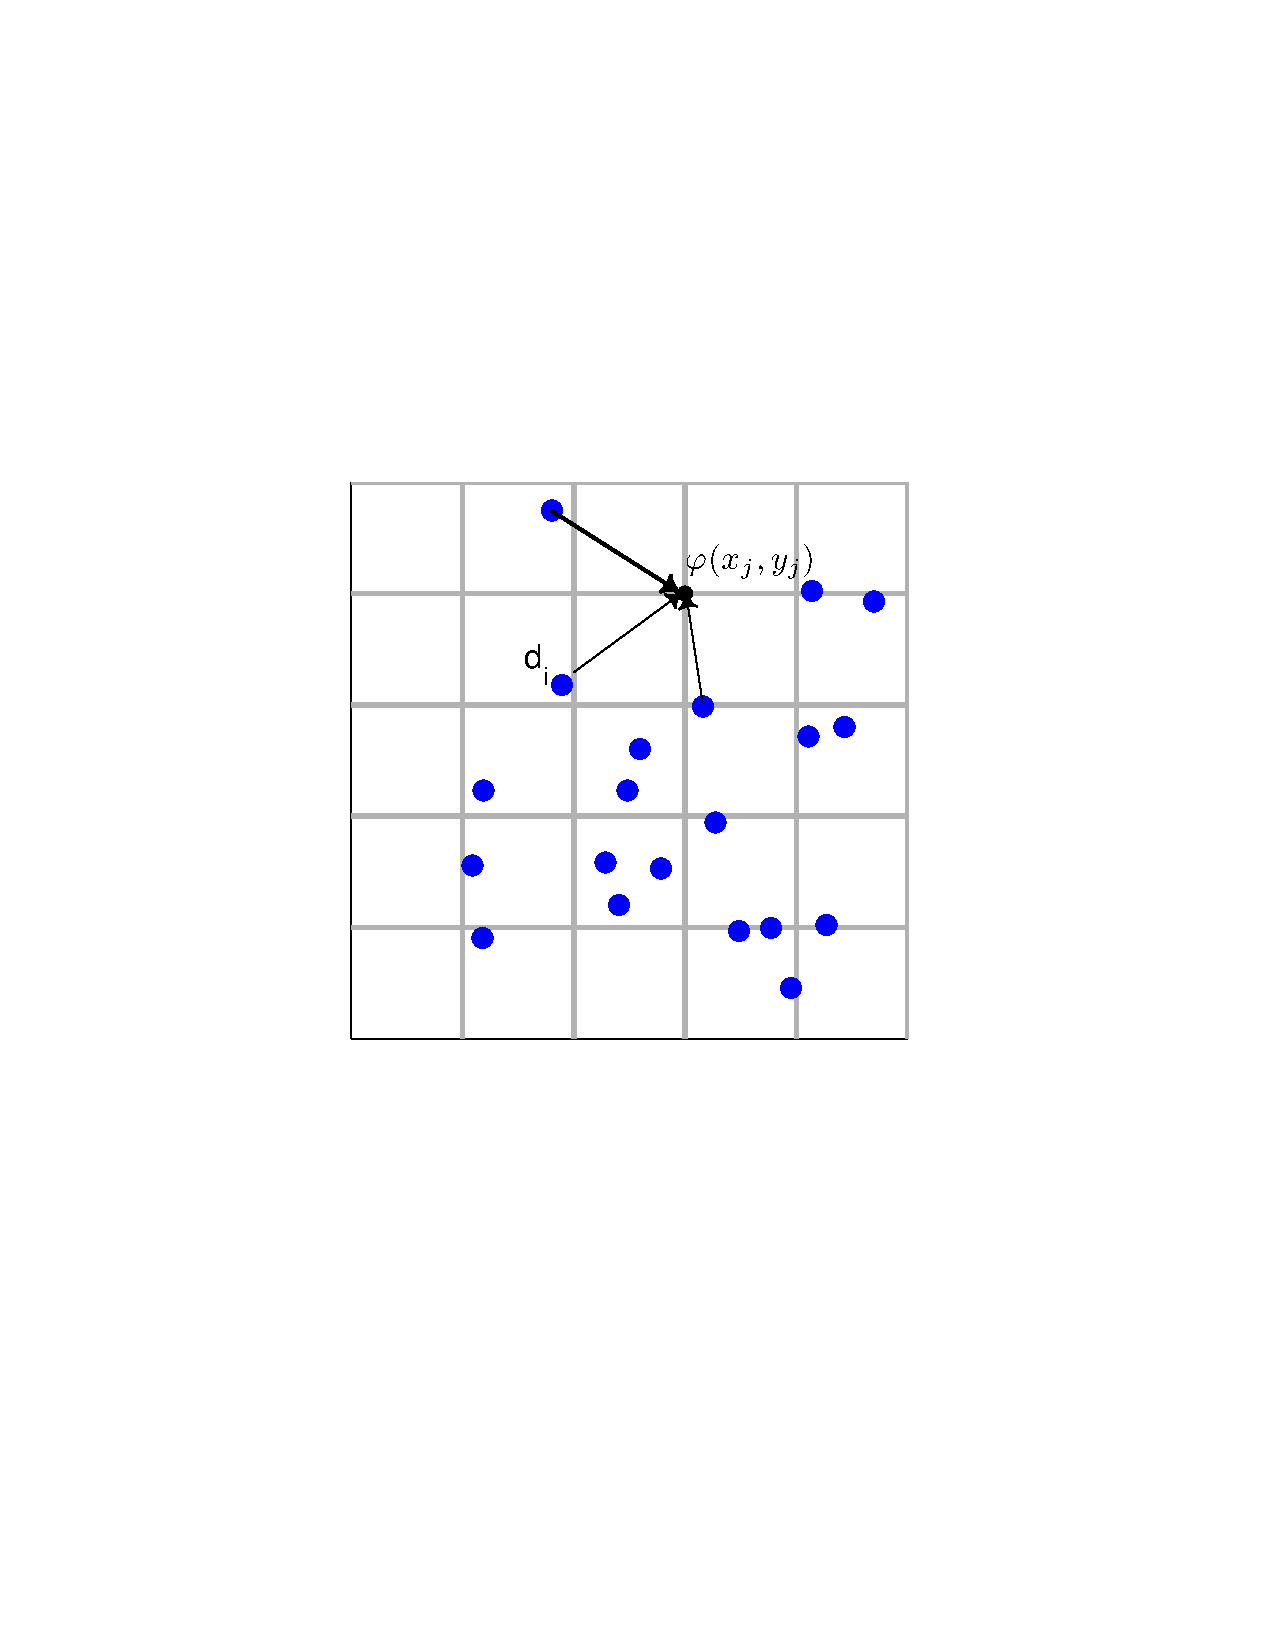
\includegraphics[width=.4\textwidth,viewport=166   289   440   564]{gridding}
\end{figure}

\important{Formulation:} minimize cost function $J[\varphi]$


\begin{eqnarray*} \label{eqn:divaJ}
& &\min {J}[\varphi] = \sum_{i=1}^{N}\mu_i \left[d_{i}-\varphi(x_{i},y_{i})\right]^{2} \onslide<2->{\qquad\textcolor{gray}{\textrm{data--analysis misfit}}}\\
	  &+& \int_{{D}}\left(
{\nablab}{\nablab}\varphi : {\nablab}{\nablab}\varphi + { \alpha_{1}}
{\nablab}\varphi \cdot {\nablab}\varphi + \alpha_{0} \varphi^{2} \right) \ddiff {D} \onslide<2->{\qquad\textcolor{gray}{\textrm{field regularity}}}
\end{eqnarray*}

\end{frame}


%-----------------------------------------------------------------------------------------
\begin{frame}[t]
\frametitle{Analysis parameters are related to data}
\footnotesize

Non-dimensional version:

\begin{eqnarray}
L  = \textrm{length scale} &\rightarrow & \tilde{\nablab} = L \nablab\\
                     	   &\rightarrow & D = L^2 \tilde{D}
\end{eqnarray}

\onslide*<2->{
\begin{eqnarray*}
\tilde{J}[\varphi]&=&\sum_{i=1}^{N}\textcolor<5>{blue}{\mu_i L^2} [d_{i}-\varphi(x_{i},y_{i})]^{2}\\ 
&+&  \int_{\tilde{D}}\left(
 \tilde{\nablab}\tilde{\nablab}\varphi : \tilde{\nablab}\tilde{\nablab}\varphi + { \textcolor<4>{blue}{\alpha_{1}} L^2}
\tilde{\nablab}\varphi \cdot \tilde{\nablab}\varphi + \textcolor<3>{blue}{\alpha_{0}} L^4 \varphi^{2} \right) \ddiff \tilde{D}\nonumber
\end{eqnarray*}
}

\onslide*<3-5>{
\begin{itemize}
\item<3-> $\alpha_0$ \fleche $L$ for which data anomaly term $\simeq$ regularity term: \hspace*{\fill} $\alpha_0 L^4 = 1$

\item<4-> $\alpha_1$ \fleche influence of gradients: \hspace*{\fill}  $\alpha_1 L^2 = 2 \xi, \qquad \xi=1$

\item<5-> $ \mu_i L^2$ \fleche weight on data: \hspace*{\fill} 
$\displaystyle \mu_i L^2= 4 \pi \frac{\textrm{signal}}{\textrm{noise}_{i}}$
\end{itemize}
}

\onslide*<6>{
Coefficients $\alpha_0$, $\alpha_1$ and $\mu_i$ related to
\begin{enumerate}
\item Correlation length $L$
\item Signal-to-noise $\snr$
\item Observational noise standard deviation $\noise_i^2$
\end{enumerate}
}
\end{frame}

%---------------------------------------------------------------------------
\begin{frame}
\frametitle{Main analysis parameters}

\begin{columns}[totalwidth=\textwidth]
\column{.5\textwidth}
\important{Correlation length $L$:}

\begin{itemize}
\footnotesize
\item[]
\item Measure of the \textit{influence} of data points
\item Estimated by a least-square fit of the covariance function
\item[]
\end{itemize}

\important{Signal-to-noise ratio $\snr$:}

\begin{itemize}
\footnotesize
\item[]
\item Measure of the \textit{confidence} in data 
\item Estimated with Generalized Cross Validation techniques
\end{itemize}

\column{.5\textwidth}

\end{columns}
\end{frame}

%-------------------------------------------------------------------------------
\begin{frame}
\frametitle{Correlation function}

In variational analysis, the correlation function is not specified
\texttt{a priori}, but its form is determined by the differential in
equation \eqref{eqn:divaJ}. For an infinite domain, one can show that
for $\alpha_0 = L^{-4}$ and $\alpha_1 = 2 L^{-2}$ 
the correlation function is given by: %\citep{BRAS96}

\begin{equation}
C(r) = \frac{r}{L} K_1 \left(\frac{r}{L}\right)
\end{equation}

where $r$ is the Euclidean distance, $L$ is the correlation length and
$K_1$ is the modified Bessel function. %\citep{ABRA64}

\end{frame}

%-------------------------------------------------------------------------------

\begin{frame}
\frametitle{Correlation function}

Correlation functions can be examined by analysing a single point with high signal-to-noise ratio and no background field (Fig.~\ref{singleanalysis}). In this particular case, we performed an analysis with a point located at the center $(0,0)$ of a square domain. The correlation length is equal to $1$ and the signal-to-noise ratio is taken equal to $1000$.

\begin{figure}[htpb]
	\centering
	\parbox{.6\textwidth}{
		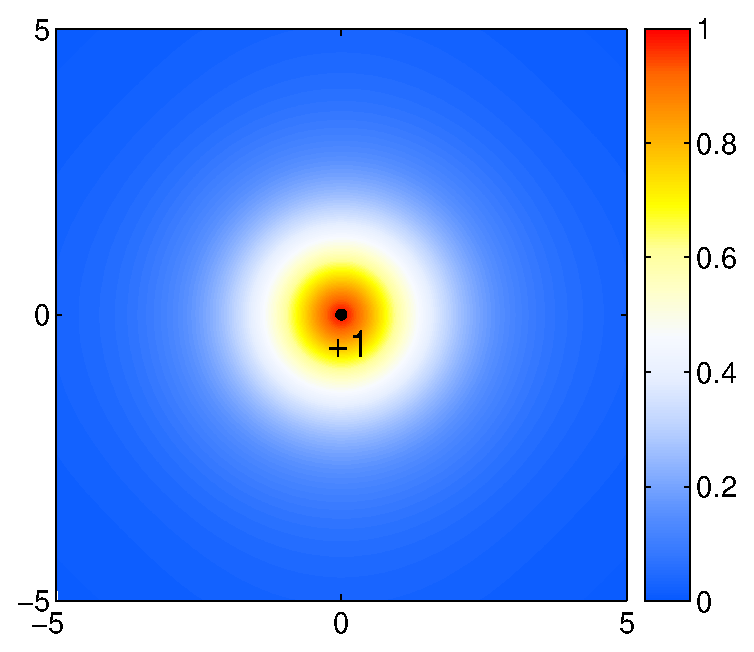
\includegraphics[width=.55\textwidth,bb=148 269 507 577]{results_test1}
		}\parbox{.4\textwidth}{
		\caption{Analysis of a single data point with high signal-to-noise ration and no background field.\label{singleanalysis}}}
\end{figure}

\end{frame}

%-------------------------------------------------------------------------------

\begin{frame}
\frametitle{Correlation function}

Figure~\ref{kernel1} shows both the exact solution and the correlation function by a single point analysis. The two curves are close to each other, the differences between the two curves being only due to the boundaries.

\begin{figure}[htpb]
	\centering
	\parbox{.6\textwidth}{
		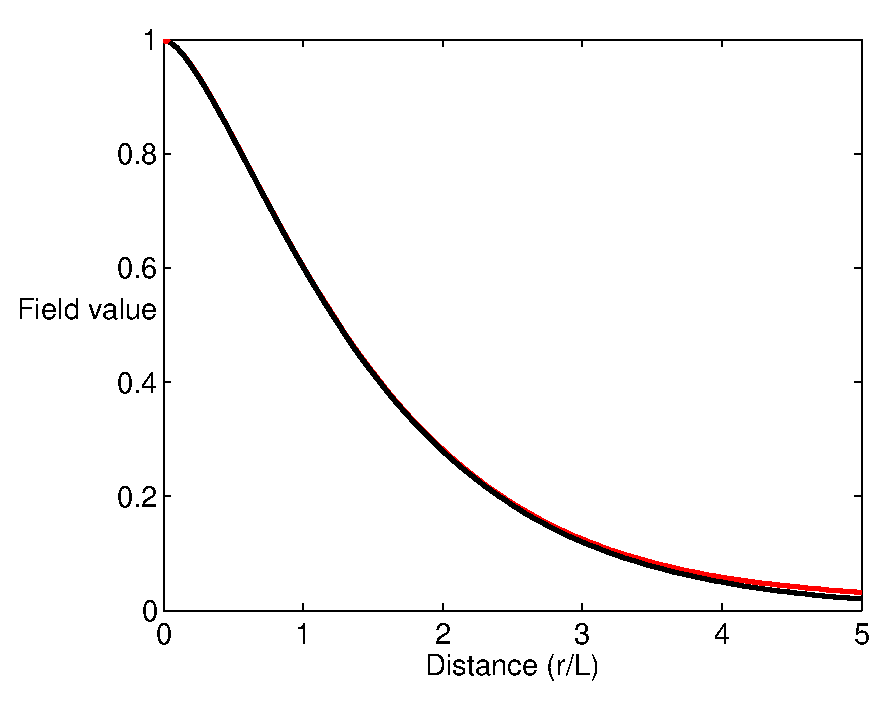
\includegraphics[width=.55\textwidth,bb=50 25 450 300]{kernelf}
		}\parbox{.4\textwidth}{
		\caption[Theoretical Kernel function and analysis of a single point with a unit value.]{The theoretical Kernel function is given in red, while the black curve comes from the analysis of a single point with a unit value.\label{kernel1}}}
\end{figure}

The Kernel function can be used to calibrate \diva parameters ($\alpha_0, \alpha_1, \mu$) so as to fit observed covariance functions. This principle is used by the tool \command{divafit} which helps one to estimate the correlation length.

\end{frame}

%-------------------------------------------------------------------------------

%\begin{frame}
%\frametitle{Correlation function}

%\centerline{\includegraphics[width=0.9\textwidth]{besselvsonepoint}}

%\end{frame}

%-------------------------------------------------------------------------------

\begin{frame}{Illustration of covariance functions}
\vspace{-0.5cm}
\begin{figure}[H]
\begin{center}
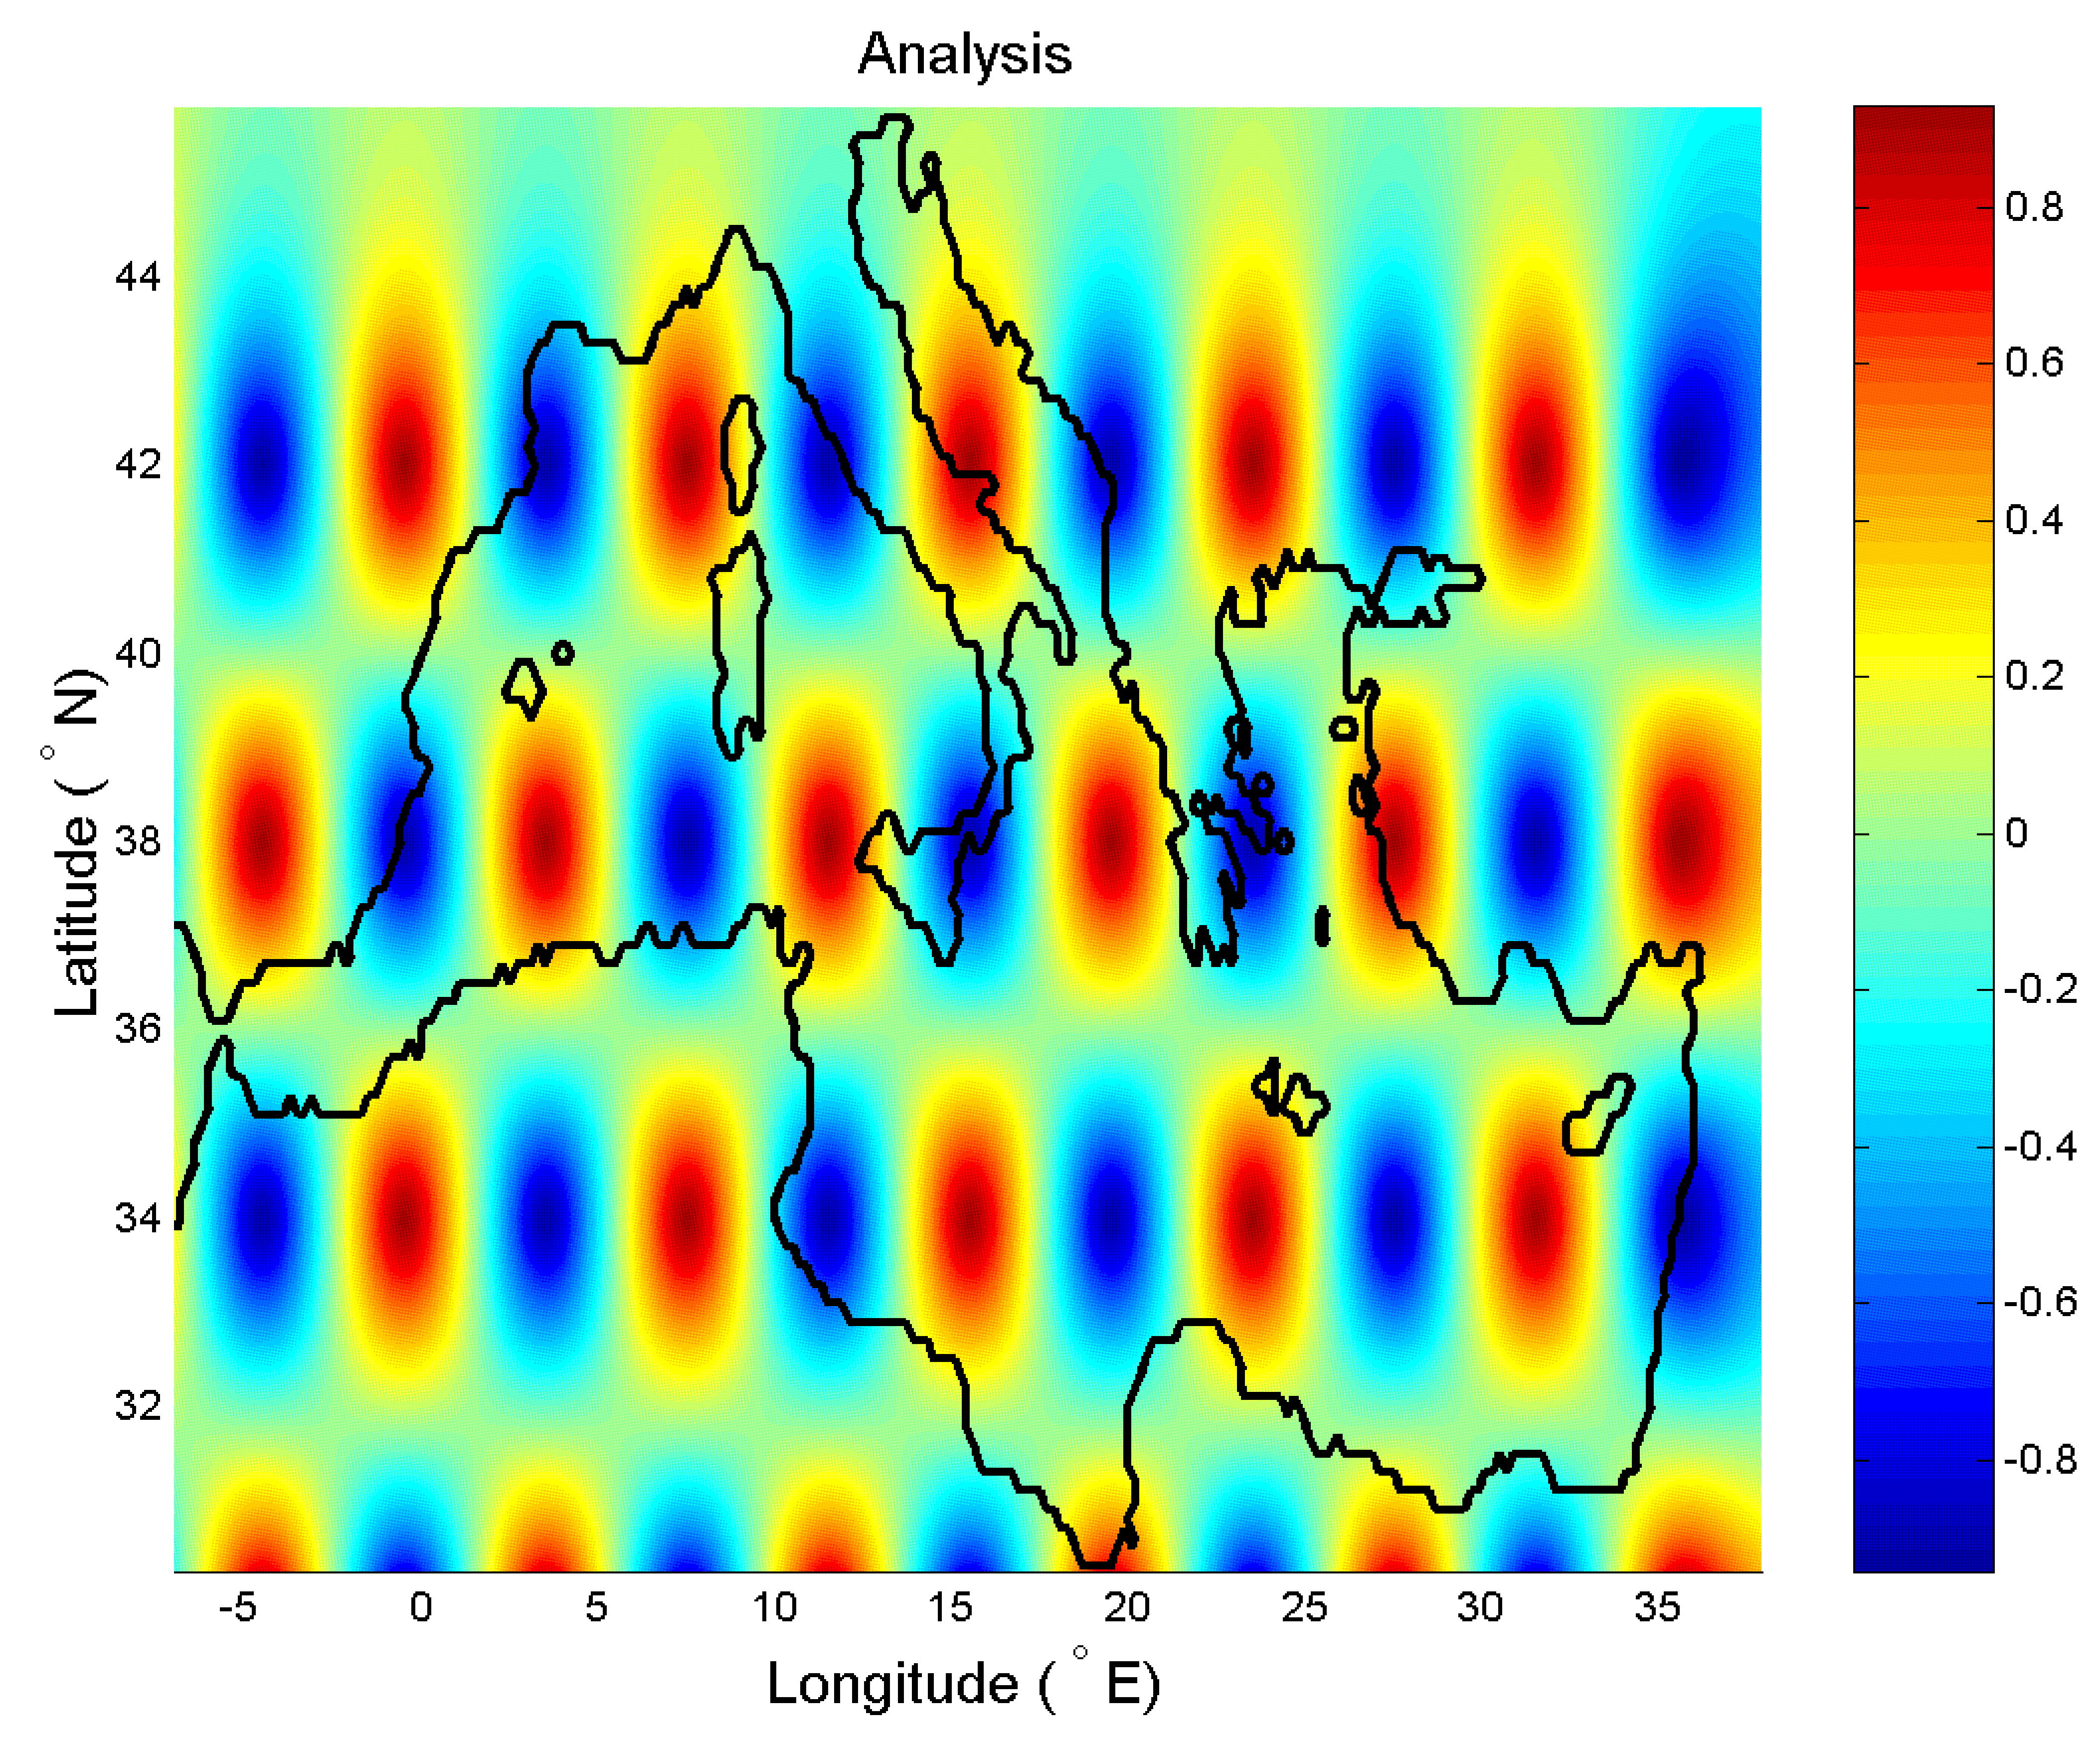
\includegraphics[width=8cm,height=4cm]{medregiso}
\vspace{0cm}
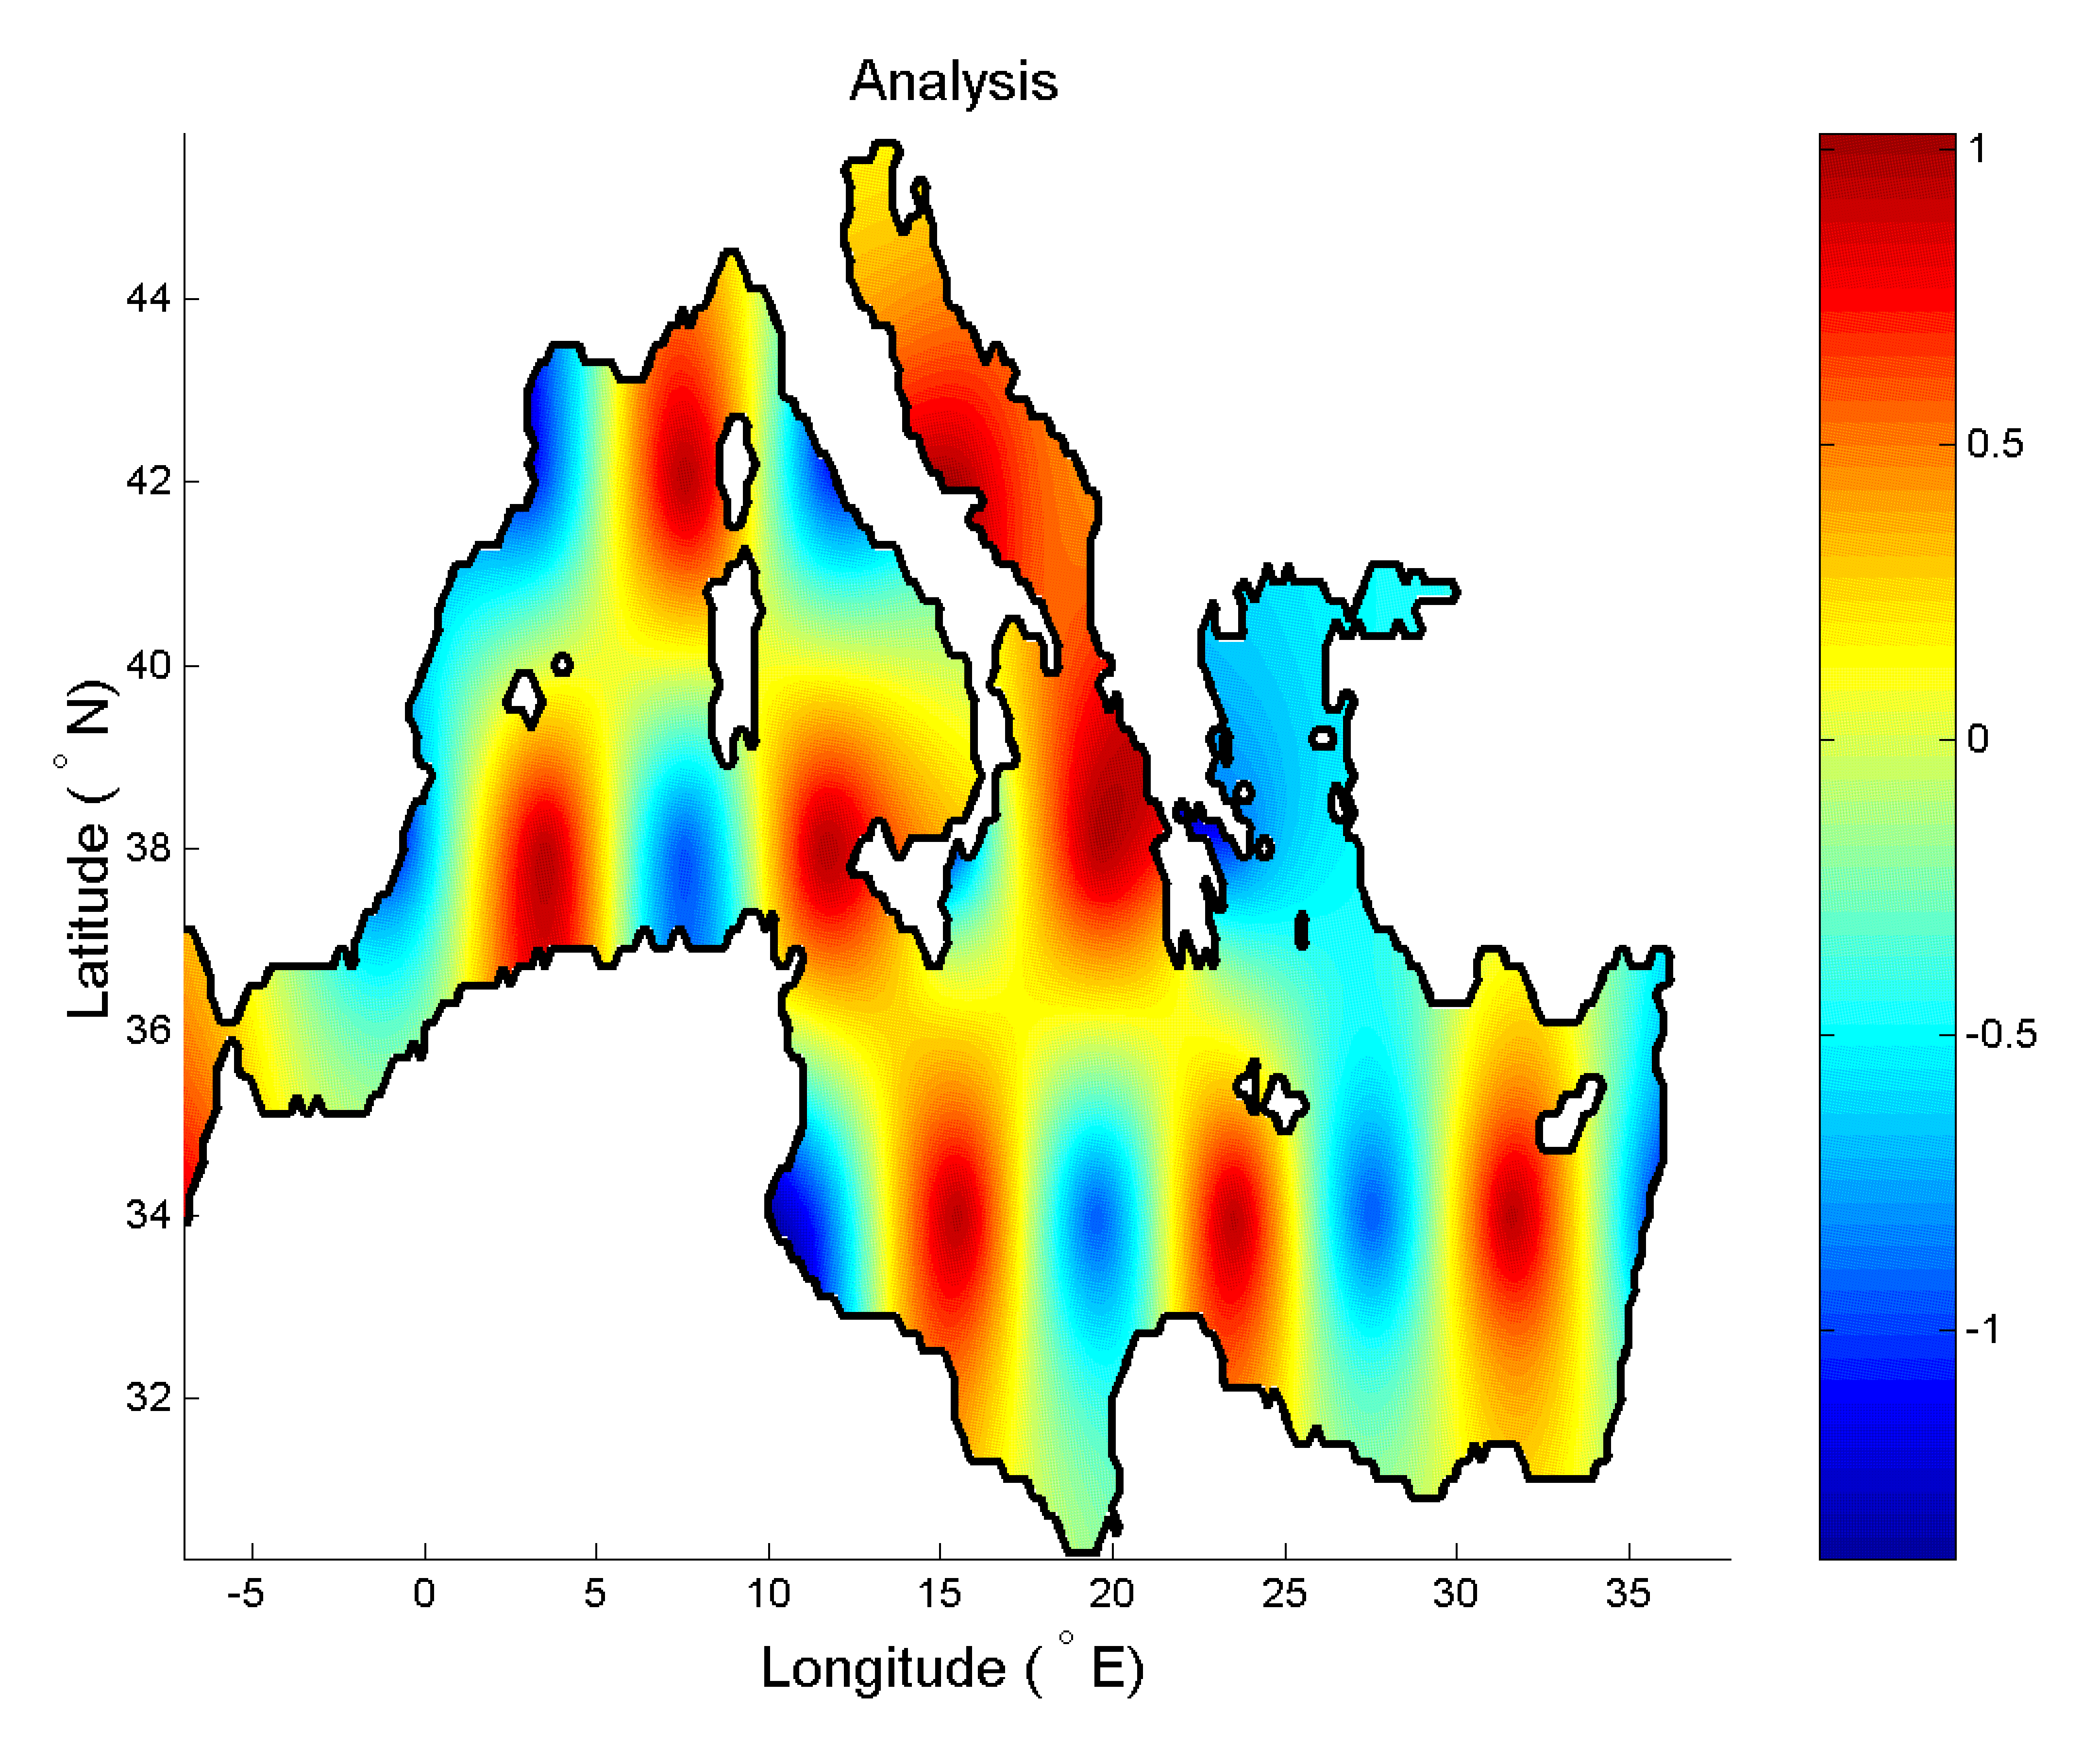
\includegraphics[width=8cm,height=4cm]{medregtopo}
%\caption{Left: data influence of alternating anomalies assuming isotropic and homogeneous covariances (typically OI approach). Right: With DIVA, data influence is not %crossing land without requiring a specific formulation in the covariance function. The finite element mesh naturally creates some decoupling.}
\end{center}
\end{figure}

\end{frame}

%-------------------------------------------------------------------------------

\begin{frame}
\frametitle{Parameter calibration : L}

\begin{figure}[H]
\centerline{
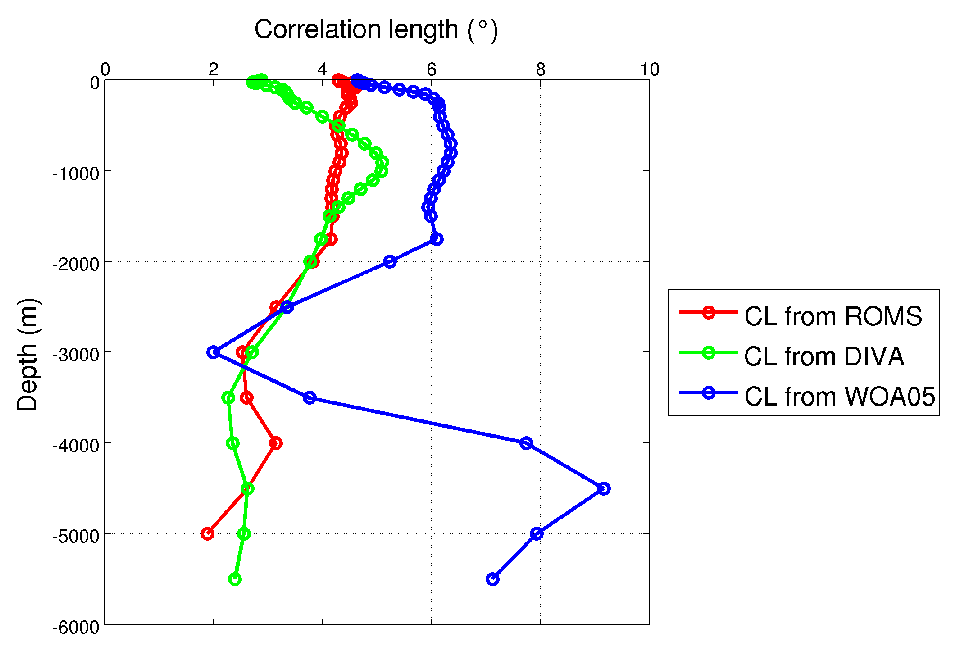
\includegraphics[height=4cm]{CL} 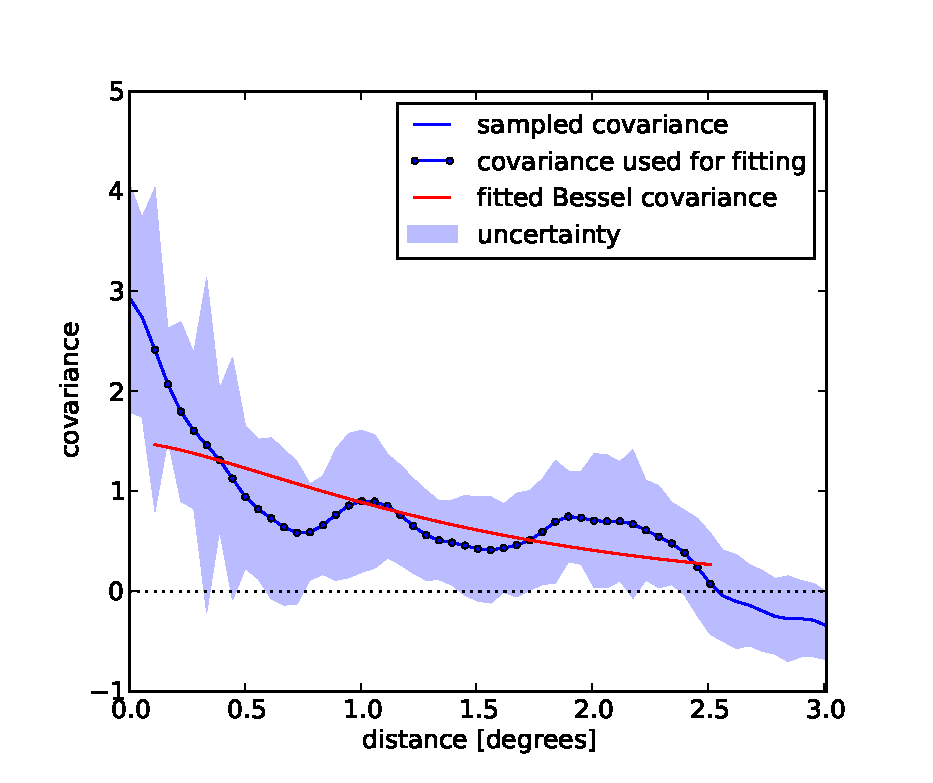
\includegraphics[height=4cm]{diva_covafit.eps}
}
% Add divafit image
\caption {Spatial coherence of parameters: here correlation length obtained with covariance fitting  
(Troupin {\it et al.}, 2010).}
\end{figure}

\end{frame}

%---------------------------------------------------------------------

\begin{frame}[allowframebreaks]
\frametitle{Parameter calibration : SNR}
\framesubtitle{Generalities}

Let us consider the vector $\vect{d}$ containing the $N$ data anomalies. Objective analysis of $\vect{d}$ leads to analysed field with minimal expected error variance. The analysis $\varphi^a$ at any location $\vect{r}$ is given by
\begin{equation}
\varphi^a(\vect{r}) = \vect{c} \inv{(\matr{B}+\matr{R})} \matr{d}
\end{equation}
where $\vect{c}$ is a vector containing the background covariance between the point in which the analysis is to be performed and all data point locations. The optimal interpolation is based on the \textit{background covariance} matrix $\matr{B}$ and \textit{error covariance} matrix $\matr{R}$ of the data.
 
Let us call $\tilde{\vect{d}}$, the analysis vector at data points. The two vectors ${\vect{d}}$ and $\tilde{\vect{d}}$ can be related by the expression:

\begin{equation}
\tilde{\vect{d}}  =  \matr{A} \vect{d}
\end{equation}

where the matrix $\matr{A}$, used to perform the analysis at the data points, is calculated according to 

\begin{equation}
\matr{A}=\matr{B} \inv{(\matr{B}+\matr{R})}.
\end{equation}

The \textit{data-covariance} matrix is the statistical average $\mean{\quad}$ of data products:

\begin{equation}
\mean{\vect{d} \, \transp{\vect{d}}} = \matr{B}+\matr{R}, 
\label{eq:datavar}
\end{equation}
where $\transp{\,}$ it the transposed matrix or vector. For uncorrelated observational errors, error-covariance matrix $\matr{R}$ is diagonal, with a variance $\noise_i^2$ for point $i$, \textit{i.e.}

\[
\matr{R} = \mathrm{diag}(\noise_i^2)%\quad\textrm{or}\quad R_{ij}= \noise_i^2\delta_{ij}.
\]

In that case, we can show that the variance of expected misfit at point $i$ is
 
\begin{equation}
\mean{\left(d_i - \tilde{d}_i\right)^2} = \noise_i^2 (1 - A_{ii}).
\label{eq:epsilonmisfit}
\end{equation}

In practice covariance matrices are known only imperfectly: their structure is often considered to be
fixed, but with imperfectly known amplitude. In other words it is often assumed that


\end{frame}

%---------------------------------------------------------------------

\begin{frame}{Parameter calibration : SNR}
\framesubtitle{Generalities}

\begin{equation}
\matr{B}= \sigma^2 \tilde{\matr{B}}
\end{equation}
\begin{equation}
\matr{R}= \epsilon^2 \tilde{\matr{R}}
\end{equation}
\begin{equation}
\matr{c}= \sigma^2 \tilde{\matr{c}}
\end{equation}
with non-dimensional correlation matrixes $\tilde{\matr{B}}$, $\tilde{\matr{R}}$, $\tilde{\matr{c}}$
\begin{equation}
\phi= {\tilde{\matr{c}}}^t \inv{\left( \tilde{\matr{B}} + {1 \over \lambda} \tilde{\Rerr} \right)} 
\observation
\label{eq:analyzedfield}
\end{equation}
with signal-to noise ratio
\begin{equation}
\lambda= {\sigma^2 \over \epsilon^2}
\end{equation}
Also the error field is only depending on the ratio.
\end{frame}

%-------------------------------------------------------------------------------§

\begin{frame}[allowframebreaks]{Parameter calibration : SNR}
\framesubtitle{Ordinary Cross Validation (OCV)}

The objective is to optimize the parameter $\snr$ by searching for its value for which the analysis has a minimal error. For this reason, we need to find a proxy norm that we will be able to minimize. As the difference of the analysis with the true field is not available, we could try to work with the difference of the analysed field at the data points with respect to the original data field:

\begin{equation}
{\theta_i^2} = {(d_i - \tilde{d}_i)^2}.
\end{equation}

If we try to minimize this norm, we will get an infinite signal-to-noise ratio and a perfect data-analysis fit. This is because the analysis at the data point is directly influenced by the corresponding data. 

\begin{itemize}
\item To avoid this inconvenience, the solution is to calculate the difference of the data value with respect to the analysed field in which the data under investigation was not taken into account. This is called the \textit{Ordinary Cross Validation} and is, with a practical trick, implemented in \command{divacv}. To make this estimate robust, the analysis has to be repeated over a large number of data points, increasing the computing cost, so that OCV is generally too expensive to perform unless a trick as in \command{divacv} can be used (there the analysis can be done without actually disregarding a data point but by correcting the difference).
 
\item Variants of OCV take out several points at once to calculate error estimates and repeat the exercise several times to make estimates robust.  In \diva this options are available in \command{divacvrand}. A variant is \command{divacvclasses} in which all data from a given class (e.g. specific year) are set aside and the analysis compared to.
\end{itemize}

\end{frame}

%-------------------------------------------------------------------------------§

\begin{frame}{Parameter calibration : SNR}
\framesubtitle{Generalised cross validation (GCV)}

According to Craven and Wahba (1978), modifying the error estimate as follows:

\begin{equation}
{\hat{\theta}_i^2} =  \frac{(d_i - \tilde{d}_i)^2}{(1 - A_{ii})^2}.
\label{eq:misfitestimate}
\end{equation}

allows one to keep the data during the analysis and will reduce the computing cost. In this formulation, the denominator penalizes more heavily data points in which the analysis is forced to be close the data and accounts therefore for the self-influence of the data point (which is absent in the case of pure cross-validation).

\end{frame}

%-------------------------------------------------------------------------------

\begin{frame}{Parameter calibration : SNR}
\framesubtitle{Computation of $A_{ii}$}

When the matrix $\matr{A}$ is not explicitly calculated, $A_{ii}$ can be obtained by performing an analysis with a vector $\vect{e}_i=(0\,0\ldots\,0\,1\,0\ldots 0)$ (zero on all data locations, except at point $i$, where its value is one). This demands an analysis for every data point in which the estimator is constructed.  

The associated computational cost can be reduced by replacing $A_{ii}$ by the average value and assuming:
\begin{equation}
A_{ii} \simeq \frac{1}{N} \trace{\matr{A}}.
\label{eq:aiitrace}
\end{equation}

\end{frame}

%-------------------------------------------------------------------------------

\begin{frame}{Parameter calibration : SNR}
\framesubtitle{Computation of $A_{ii}$}

To avoid calculating all $A_{ii}$ and summing them up, we can use the following estimate (Girard, 1989):
\begin{equation}
\frac{1}{N} \trace{\matr{A}} \simeq  \frac{ \transp{\vect{z}} \matr{A} \vect{z} }{\transp{\vect{z}} \vect{z} }
\label{eq:traceest}
\end{equation}
where $\vect{z}$ is a vector of random variables of zero mean. For robustness, the trace estimate can be repeated several times with different random vectors, averaging of the different estimates. The number of estimates is the parameter provided to the module \texttt{GCVFAC} of \diva.

\end{frame}

%-------------------------------------------------------------------------------

\begin{frame}{Parameter calibration : SNR}
\framesubtitle{Generalized cross validator}

In order to make the error estimator robust, we take the average over all data points and define the \textit{generalized cross validator} as 
\[
\Theta^{2}=\frac{1}{N}\sum_{i=1}^{N}\hat{\theta}_i^2.
\] 
Assuming temporarily $\noise_{i}^{2} = \noise^{2}$, hence having all misfits with the same weight, the generalized cross validator is obtained:

\begin{equation}
\Theta^2=\frac{\vnorm{\vect{d}-\tilde{\vect{d}}}^2}{N \left(1- \frac{1}{N}\trace{\matr{A}}\right)^2} 
        =\frac{\vnorm{(\matr{I}-\matr{A})\vect{d}}^2}{(1/N)\left(\trace{\matr{I}-\matr{A}}\right)^2}
\label{eq:gcv}
\end{equation}

The GCV consists in minimizing $\Theta^{2}$ by changing the signal-to-noise ratio $\snr$. $\Theta^2$ is a global estimate of the analysis error variance.

\end{frame}

%-------------------------------------------------------------------------------§

\begin{frame}{Parameter calibration : SNR}
\framesubtitle{Generalized cross validator}

Defining the diagonal matrix $\matr{W} = \diag(w_i)$, the generalized cross validator then reads:

\begin{equation}
\Theta^2=\frac{ \transp{\left(\vect{d}-\tilde{\vect{d}}\right)} \matr{W} \left(\vect{d}-\tilde{\vect{d}}\right) }{ N \left(1 - \frac{1}{N}\trace{\matr{A}}\right)^2} 
\label{eq:gcvbis}
\end{equation}

where the weights should satisfy

\begin{equation}
\sum_i \frac{1 }{w_i} = N.
\label{eq:condition}
\end{equation}

The $\tilde{w}_i$ are the values provided as optional fourth column in \file{data.dat}.

\command{divacv} uses cross validation with complete calculation of $A_{ii}$, whereas \command{divagcv} uses the approximation $A_{ii} N=\trace{\matr{A}}$.

\end{frame}

%-------------------------------------------------------------------------------§
\begin{frame}
\footnotesize
\frametitle{Minimization with a finite-element method}

Field regularity \fleche plate bending problem \fleche finite-element solver

%Belgian specialties: finite-element mesh
\begin{figure}[H]
\centering
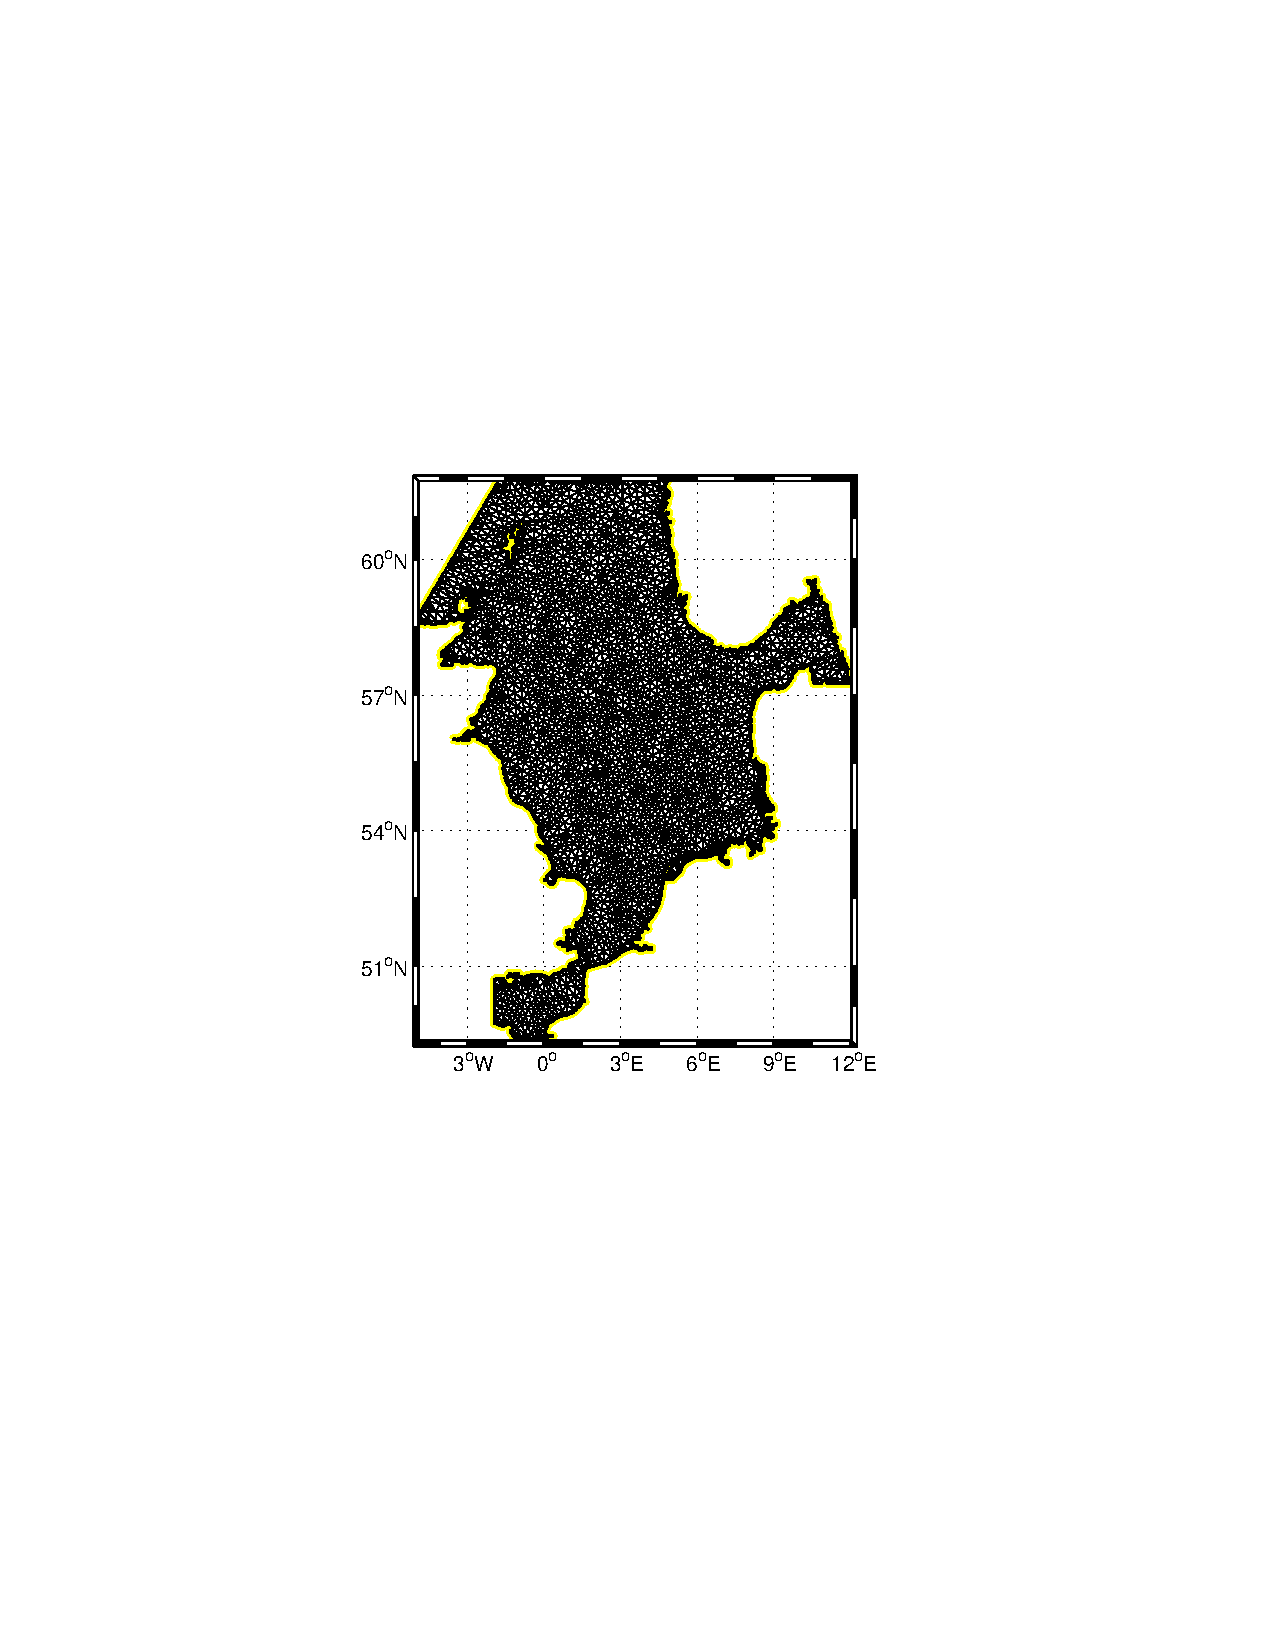
\includegraphics[width=.3\textwidth,viewport=165 273 429 567]{mesh_northsea}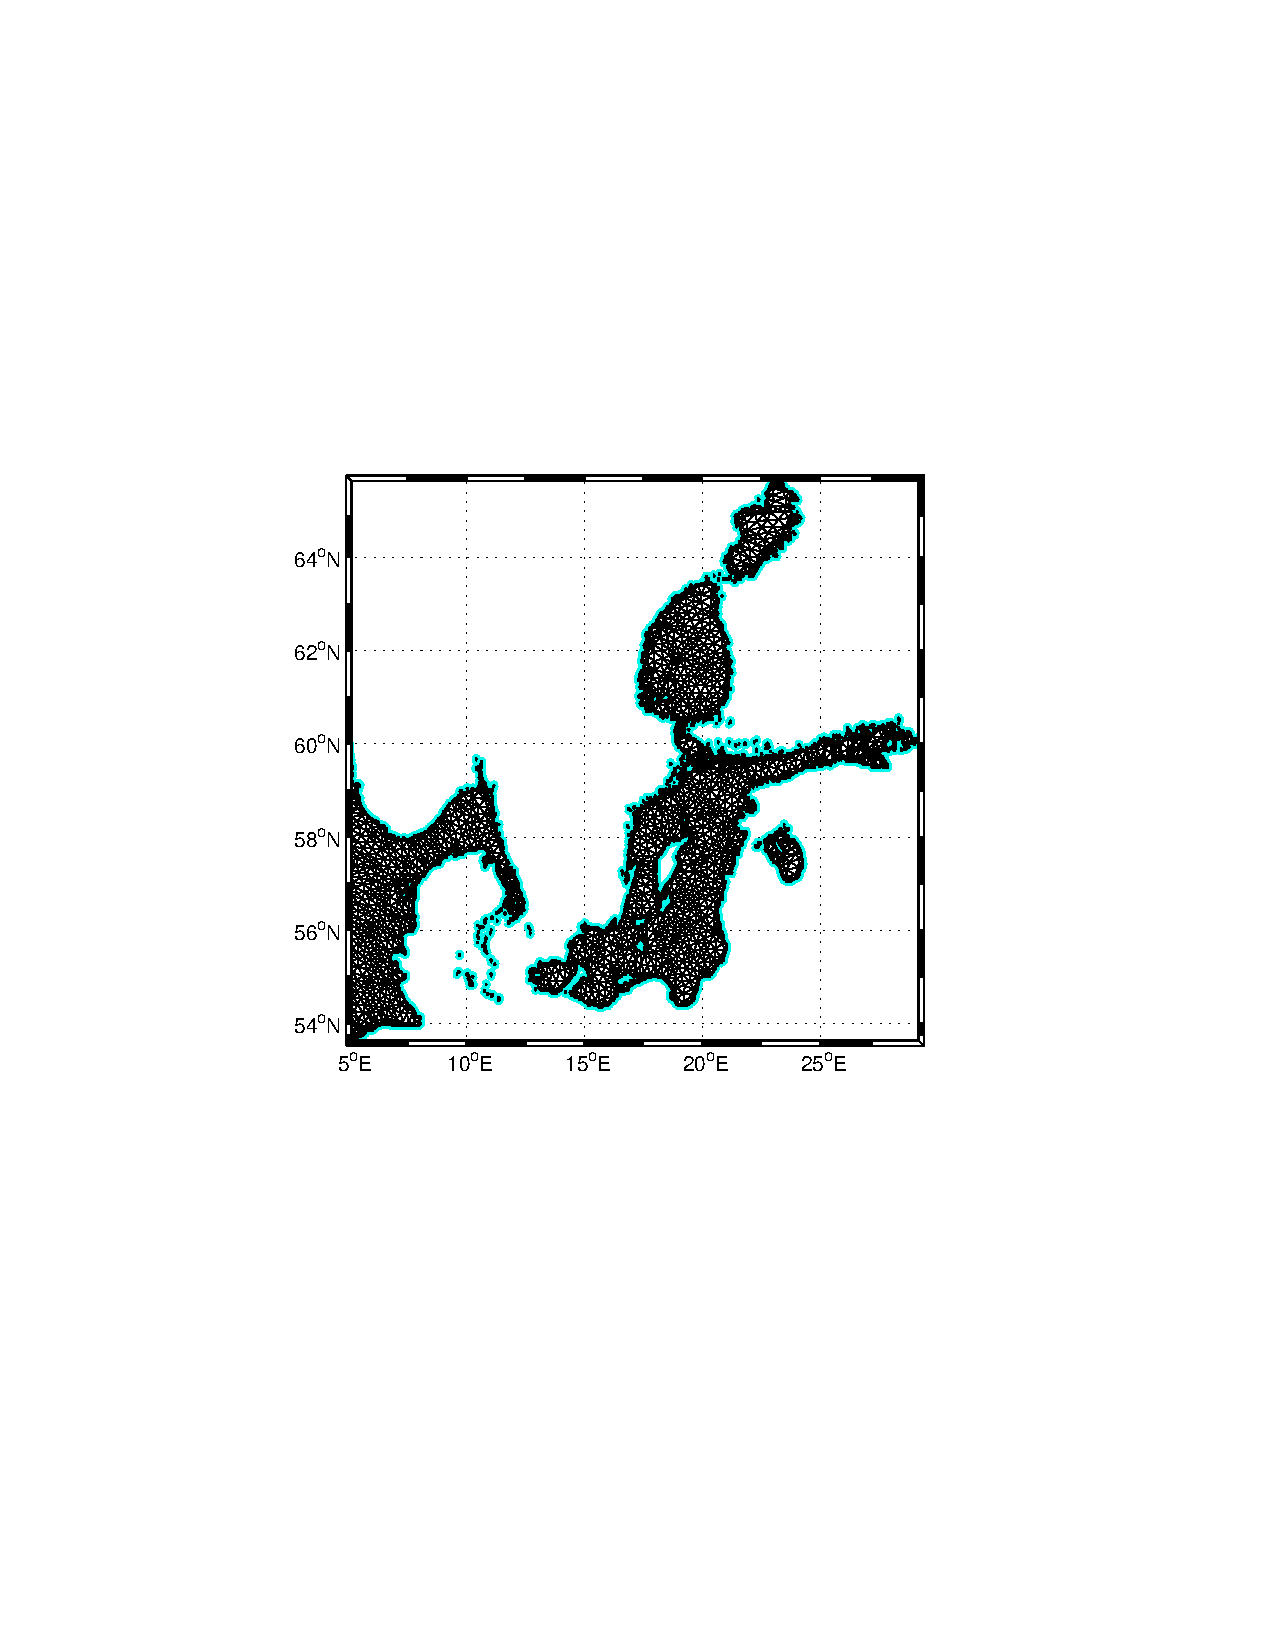
\includegraphics[width=.3\textwidth,viewport=133 272 448 568]{mesh_baltic}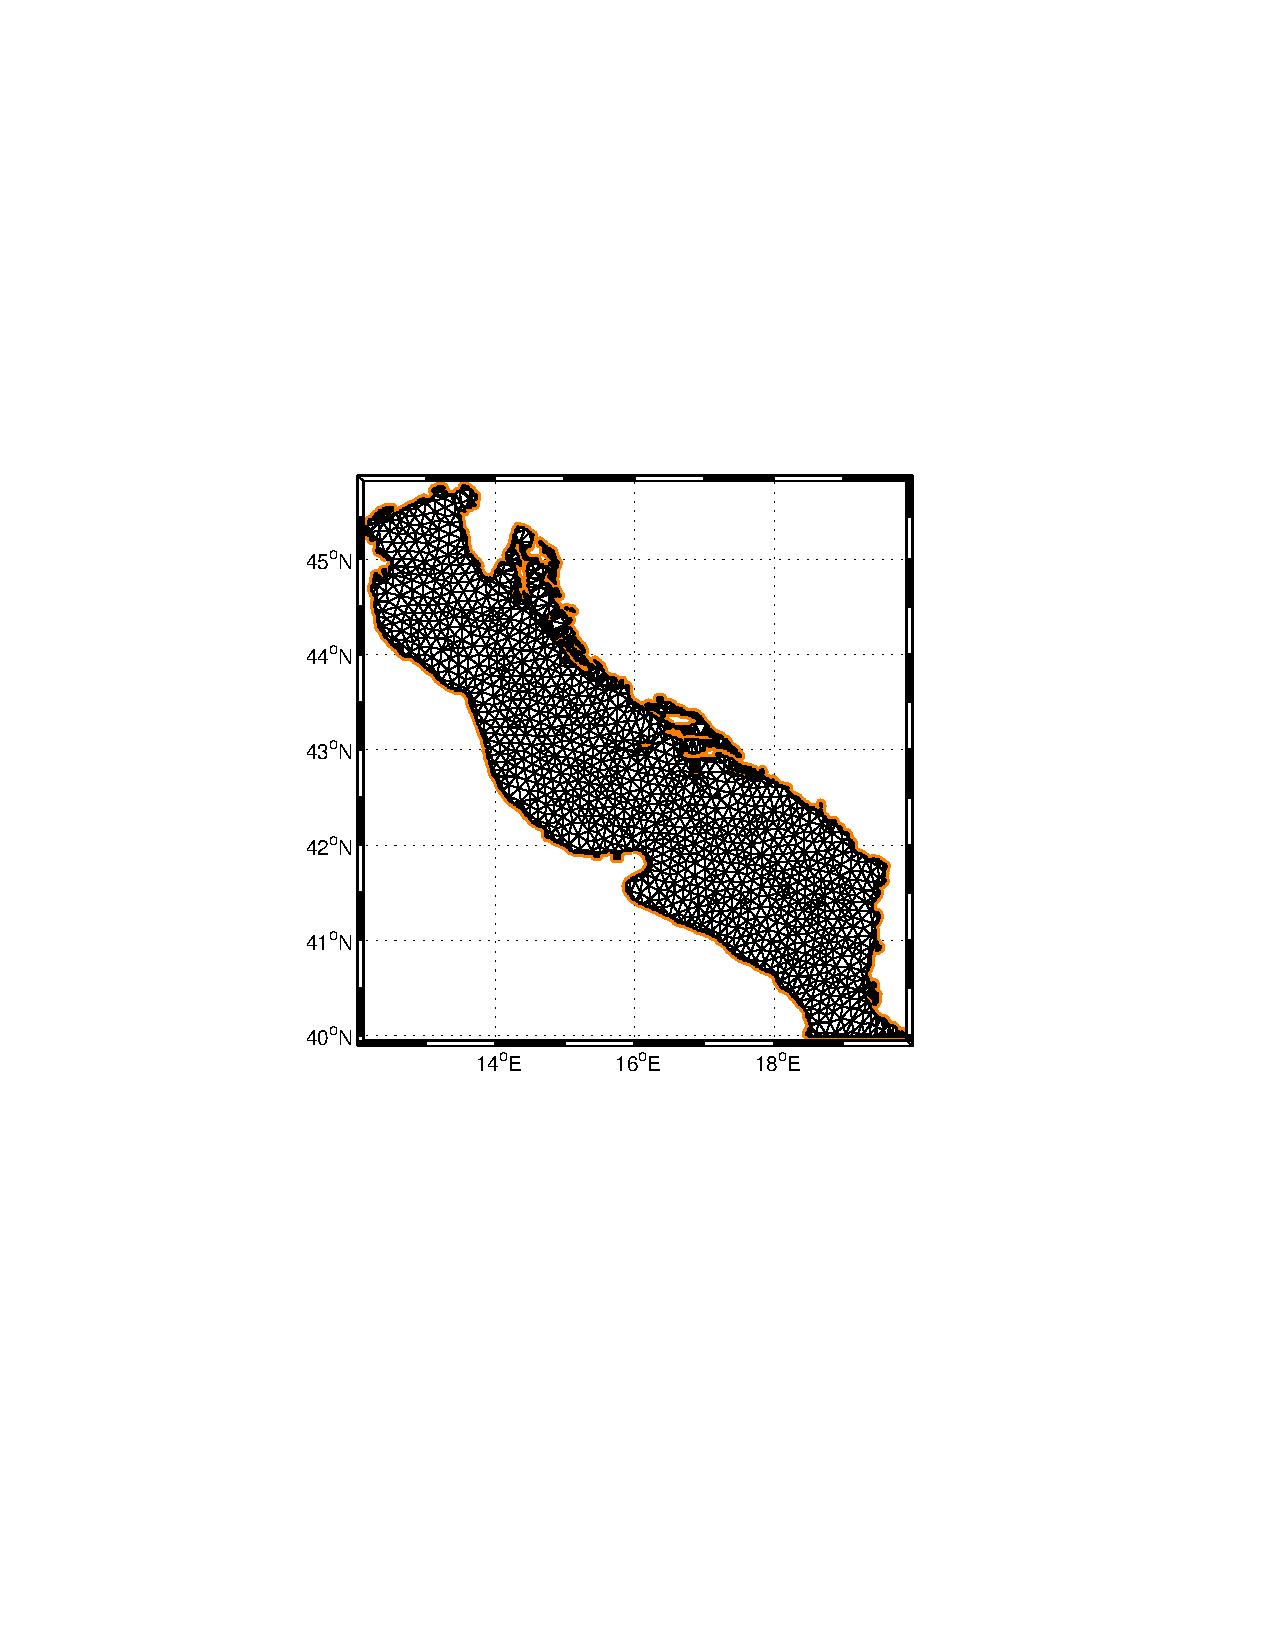
\includegraphics[width=.3\textwidth,viewport=138 272 443 568]{mesh_adriatic}
\end{figure}
\textbf{Advantages:}
\begin{itemize}
\item boundaries taken into account
\item numerical cost (almost independent on data number)
\item no \textit{a posteriori} masking (except if based on error level) 
\end{itemize}

\end{frame}

%----------------------------------------

\begin{frame}{Minimization with a finite-element method}
%\vspace{-0.5cm}
%\begin{equation}
%\mu=\frac{\sigma^{2}}{\epsilon^{2}} \frac{4 \pi}{L^{2}}
%\end{equation}
%where the $\sigma^{2}/\epsilon^{2} $  is known as a signal to noise 
%ratio $S/N$.
\centerline{
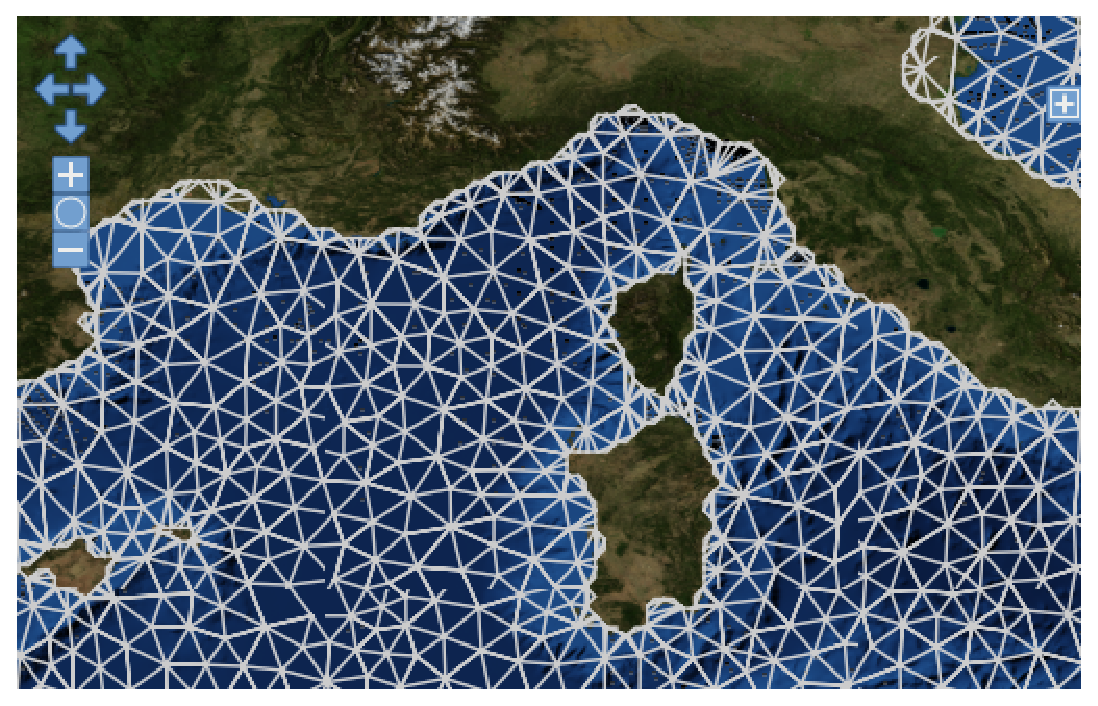
\includegraphics[width=7cm]{divamesh.eps}
}
Solution by finite element method. % including DIVA mesh generator using topographic data. 
Note decoupling of subbasins. (Each element is in fact composed by three sub-elements) %, each one with cubic functions)
\begin{itemize}
\item The solution method relies on a finite-element resolution, the mesh being automatically generated using one of the tools provided within the software. 
\item The finite element mesh only covers actual sea so that land regions are excluded from the analysis and provide natural barriers for data-information propagation.
\end{itemize}
\end{frame}

%----------------------------------------

\begin{frame}
\frametitle{Minimization with a finite-element method}
\footnotesize

%\begin{columns}[totalwidth=\textwidth]
%\column{.6\textwidth}

\onslide*<1>{

\begin{equation}
\textrm{Triangular FE only covers sea:}\qquad J[\varphi] = \sum_{e=1}^{N_{e}}J_{e}(\varphi_{e})
\label{eq:split}
\end{equation}

\begin{equation}
\textrm{In each element: } \varphi_{e}(\mathbf{r_e})=\mathbf{q_e}^{T}\mathbf{s}(\mathbf{r_e}) \quad \textrm{with} \left\{ \begin{array}{ll}
         \mathbf{s} & \rightarrow \mbox{shape functions}\\
         \mathbf{q} & \rightarrow  \mbox{\important{connectors}}\\
         \mathbf{r_e} & \rightarrow \mbox{position}
         \end{array} \right.
\label{eq:connectors}
\end{equation}

     
     
\eqref{eq:connectors} in \eqref{eq:split} + variational principle
\begin{equation}
J_{e}(\mathbf{q_e}) = \mathbf{q_e}^{T}\mathbf{K_e}\mathbf{q_e}-2\mathbf{q_e}^{T} \mathbf{g_{e}}+\sum_{i=1}^{N_{d_{e}}}\mu_{i}d_{i}
\label{eq:elements}
\end{equation}

\[ \quad\textrm{where }\left\{ \begin{array}{ll}
         \mathbf{K_e} & \rightarrow \mbox{local stiffness matrix}\\
         \mathbf{g} & \rightarrow  \mbox{vector depending on local data}
         \end{array} \right.
\]
}
      
      
\onslide*<2>{

\tikzstyle{na} = [baseline=-.5ex]
\begin{align}
\textrm{On the whole domain:}&&   J(\mathbf{q}) = \mathbf{q}^{T}\mathbf{K}\mathbf{q}-2\mathbf{q}^{T}\mathbf{g}+\sum_{i=1}^{N_{d}}\mu_{i}d_{i} &  \\
\textrm{Minimum:}&&  \mathbf{q}=\mathbf{K}^{-1}\mathbf{g}    & \\
&&    \tikz[baseline]{
            \node[fill=blue!30,anchor=base] (t1)
            {$\mathbf{q}$};
            } = 
        \tikz[baseline]{
            \node[fill=gray!30,anchor=base] (t2)
            {$\mathbf{K^{-1}}$};
        } 
        \tikz[baseline]{
            \node[fill=green!20,anchor=base] (t3)
        {$\mathbf{g}$};
        } & 
\end{align}

\begin{itemize}
\scriptsize
    \item Stiffness matrix
        \tikz[na]\node[coordinate] (n1) {};
    \item Connectors (new unknowns)
        \tikz[na]\node [coordinate] (n2) {};
    \item Charge vector
        \tikz[na]\node [coordinate] (n3) {};    
\end{itemize}
       
\begin{tikzpicture}[overlay]
\path[-] (n1) edge [out=0, in=-90] (t1);
\path[-] (n2) edge [out=0, in=-90] (t2);
\path[-] (n3) edge [out=0, in=-90] (t3);
\end{tikzpicture}

%$\mathbf{K}$ \fleche size proportional to $N_{\mathrm{dof}}$\\
%$\mathbf{K}^{-1}$ \fleche $N_{\mathrm{dof}}^{5/2}$ op. 

\begin{align*}
\textrm{Mapping of data on FEM} &\rightarrow & \textrm{transfer operator $\mathbf{T_{2}}$}&\rightarrow &\mathbf{g}=\mathbf{T_2}(\mathbf{r})\mathbf{d} \label{eq:T2}\\
\textrm{Solution at any location} &\rightarrow & \textrm{transfer operator $\mathbf{T_{1}}$}&\rightarrow &\boldsymbol{\varphi}(\mathbf{r})=\mathbf{T_1}(\mathbf{r})\mathbf{q}
%\label{eq:T1}
\end{align*}


\begin{align*}
\textrm{Results obtained at any location} \rightarrow  \boldsymbol{\varphi} = \mathbf{T_1}(\mathbf{r})\mathbf{K}^{-1}\mathbf{T_2}(\mathbf{r}) \mathbf{d} & &
%\label{eq:solution2}
\end{align*}

}
\end{frame}

%--------------------------------------------------------------------------------------------------------

\begin{frame}
\frametitle{DIVA as OI}

\vspace{-.5cm}
DIVA is identical to the well known Optimal Interpolation
%\centerline{\includegraphics[width=2cm]{../Seminars/besselvsonepoint.eps}}
\begin{itemize}
\item
if so-called reproducing kernel of the norm$~=~$ covariance function of OI, 
\item
if the noise is random, spatially uncorrelated and the signal/noise ratio parameter is identical with OI.
\end{itemize}
In this case, the OI solution$~=~$DIVA solution.
\begin{itemize}
\item Advantages of DIVA: regularization, fast finite-element solution, boundary effects taken into account.
\item Difficulties: generalizations to 3D and multivariate versions are "hybrid" (some expensive O.I. components).
\end{itemize}
% Kernel function (blue) can be "looked at" by a single point analysis with high signal/noise ratio and no background field.
% The exact function in an infinite domain is given in red and differences are only due to boundaries.
Major direct advantage of DIVA: matrix to invert is related to the finite-element mesh, NOT the number of data. Useful for large data sets (Rixen {\it et al.}, 2000).
Equivalence allows to calculate error fields with DIVA even if formulation does not rely on error minimisation.
\end{frame}

%--------------------------------------------------------------------------------------------------------

\begin{frame}{Comparison}

{\tiny{\begin{center}
\hspace*{-1cm}
\begin{tabular}{l||c|c|c|c|c|c|c|c|}
Method & $\min(\epsilon^2)$ & 3D           & Multivar & Ops/image   & $\epsilon(\vect{r})$ & a priori   & C.V.           & anisotropy      \\ \hline \hline
Cressman &                 & $\star$       &  $\star$ &  $N_d N_a$  &                      &   $w(r/L)$ &     ($L$)      &       ($\star$)  \\ \hline
O.I.     &   $\star$       & $\star$       &  $\star$ &  $N_d^3+ N_d N_a$  &     $\star$        &   $c(r/L)$ &     $L, \sigma^2/\mu^2$   &       ($\star$)  \\ \hline
%S.C.     &   ($\star$)     & $\star$       &  $\star$ &  $N_d^3 N_a$ ??  &  $\star$        &   $c(r/L)$ &     $L, n$   &       ($\star$)  \\ \hline
\shabox{{\bf DIVA} }     &   $\star$       &  ($\star$)    &  ($\star$) &  $N_e^{5/2}$  &   $\star$        &  $K(r/L)$ &     $L, \sigma^2/\mu^2$   &       $\star$  \\ \hline
DINEOF   &   ($\star$)     &  $\star$    &  $\star$ &  $N_a^{5/4}$  &   ($\star$)        &     stat.   &     $N$   &       $\star$  \\ \hline
\end{tabular}
\end{center}
\begin{itemize}
\item[$N_d$]: number of data points
\item[$N_a$]: number of grid points for analysis
\item[$N_e$]: number of finite elements
\item[$N$]: number of EOFs
\item[$L$]: correlation length
\item[$\sigma^2/\epsilon^2$]: signal to noise ratio
\item[$\star$]: available feature
\item[($\star$)]: available with some adaptations\hypertarget{COMPARE}{}
\end{itemize}
}}
\end{frame}

%--------------------------------------------------------------------------------------------------------

\begin{frame}[t]
\frametitle{Diva Cocktail Recipe}

\begin{columns}[totalwidth=1.\textwidth]
\column{.65\textwidth}
\important{Ingredients:}
\onslide*<1>{
\begin{itemize}
\item 1 1/2 oz vodka
\item 1/2 oz passion-fruit juice
\item 1/2 oz lime juice
\item 1 tbsp cherry juice
\item fill with soda 
\end{itemize}
} 

\onslide*<2>{
\begin{itemize}
\item Smoothness \tikz[na] \coordinate (s-smooth);
\item Observation constraint \tikz[na] \coordinate (s-obs); 
\item Behaviour constraint \tikz[na] \coordinate (s-behaviour);
\end{itemize}
} 

\column{.35\textwidth}

\tikzstyle{background grid}=[draw, black!50,step=1cm]
\begin{tikzpicture}%[show background grid]
\node [inner sep=0pt,above right] 
{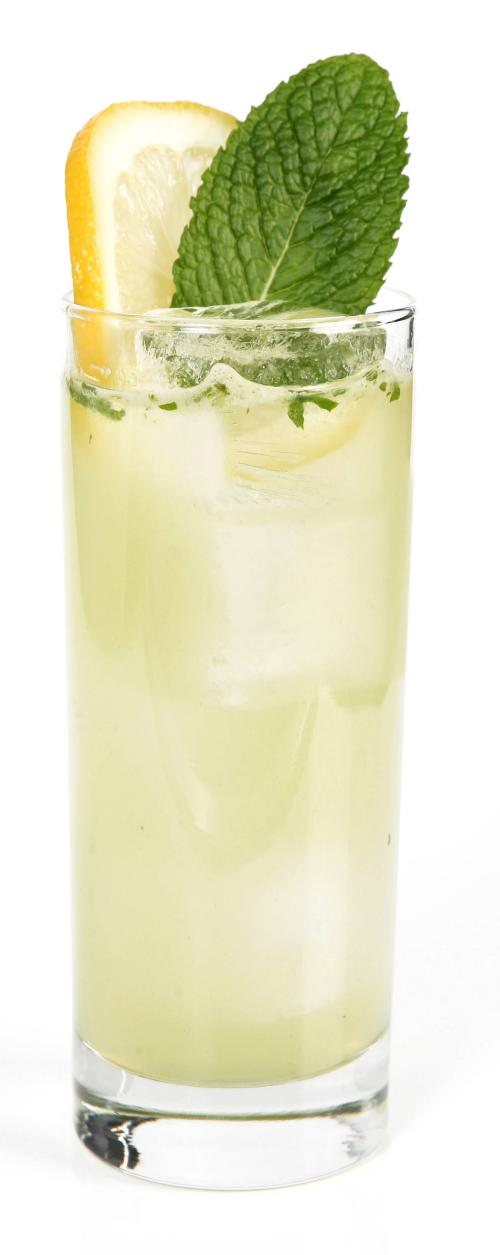
\includegraphics[width=.8\columnwidth]{cocktail}};
            % show origin
            %\fill (0,0) circle (2pt);
            % define destination coordinates
            \path (1.5,5.75) coordinate (smooth)
                  (0.4,1) coordinate (behaviour)
                  (0.4,3) coordinate (obs);
\end{tikzpicture}


\end{columns}
\onslide*<2>{
\begin{tikzpicture}[overlay]
        \path[-,black,thick] (s-smooth) edge (smooth);
        \path[-,black,thick] (s-obs) edge  (obs);
        \path[-,black,thick] (s-behaviour) edge  (behaviour);
\end{tikzpicture}
}
\end{frame}

%---------------------------------------------------------------------

\begin{frame}
\frametitle{DIVA illustration}
\centerline{
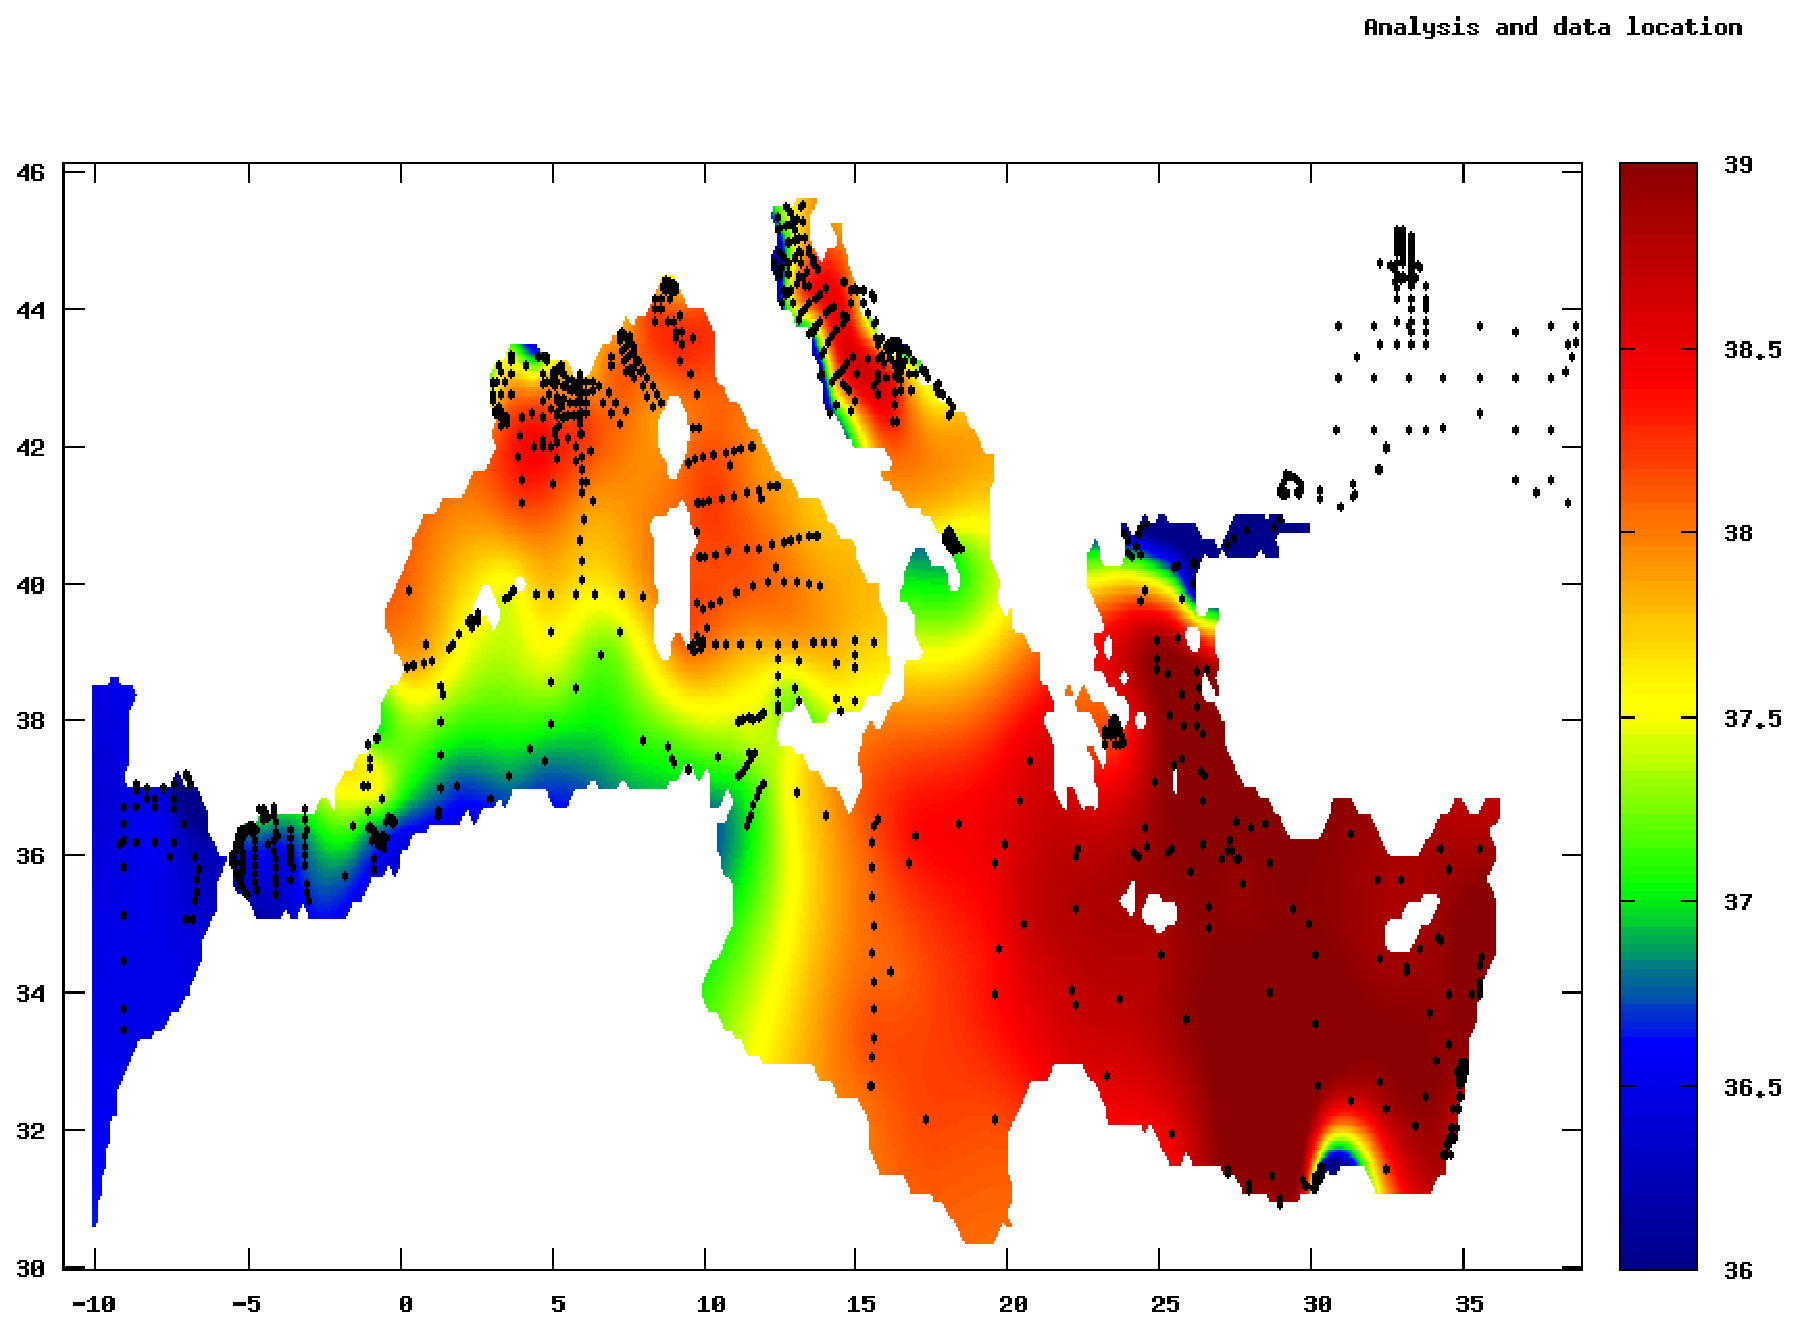
\includegraphics[width=0.9\textwidth]{diva_analysis_data}
}
\end{frame}

%---------------------------------------------------------------------------------------------------
\begin{frame}[t]

\frametitle{Want to use \diva?}

\onslide*<1>{Playing\ldots}
\onslide*<2>{With your own data\ldots} 
\onslide*<3>{For serious work: \begin{description}
\item[2D version] (for production), open source, GPL 
\item[nD version] (for research), open source, GPL
\end{description}
}

%\begin{overlayarea}{\textwidth}{6.5cm}
\begin{figure}
\centering
\includegraphics<1>[width=.625\paperwidth]{diva_demo}
\includegraphics<2>[width=.8\paperwidth]{divaonweb}
\includegraphics<3>[width=.75\paperwidth]{divascreen}
\end{figure}
%\end{overlayarea}

\onslide*<1>{\footnotesize \url{http://data-assimilation.net/Tools/divand_demo/html/}}
\onslide*<2>{\footnotesize \url{http://gher-diva.phys.ulg.ac.be/web-vis/diva.html} or ODV or matlab wrapper}
\onslide*<3>{\footnotesize \url{http://modb.oce.ulg.ac.be/mediawiki/index.php/DIVA}}
\end{frame}

%-----------------------------------------------------------------------------------------------------------
\begin{frame}[t]
\frametitle{Running \diva in 2D: input files}

\begin{overlayarea}{\textwidth}{2cm}
\begin{enumerate}
\item<1-> \file{data.dat}: contains the observations \hfill \textcolor{gray}{x|y|value}
\item<2-> \file{coast.cont}: delimits land and sea \hfill \textcolor{gray}{(coastline or isobaths)}
\item<3-> \file{param.par}: analysis parameters \hfill \textcolor{gray}{$L$, $\lambda$, resolution, \ldots}
\end{enumerate}
\end{overlayarea}

\begin{figure}
\includegraphics<1>[height=.6\textheight]{datadat}
\includegraphics<2>[height=.6\textheight]{coastcont}
\includegraphics<3>[height=.6\textheight]{parampar}

\end{figure}
\end{frame}

%-----------------------------------------------------------------------------------------------------------
\begin{frame}[t]
\frametitle{Workflow in 2D}

\begin{overlayarea}{\textwidth}{.5cm}
\onslide*<1>{Select region of study}
\onslide*<2>{Extract \important{topography}, for example via {\tiny{\url{http://gher-diva.phys.ulg.ac.be/web-vis/diva.html}}}}
\onslide*<3>{Generate \important{contour}}
\onslide*<4>{Extract \important{data}}
\onslide*<5>{Evaluate analysis \important{parameters}}
\onslide*<6>{Create finite-element\important{ mesh}}
\onslide*<7>{Generate \important{analysis}}
\onslide*<8>{Generate \important{error} field}
\end{overlayarea}

\begin{figure}
\centering
\includegraphics<1>[width=.99\textwidth]{example2D_1_bs}
\includegraphics<2>[width=.89\textwidth]{example2D_2_bs}
\includegraphics<3>[width=.99\textwidth]{example2D_3_bs}
\includegraphics<4-5>[width=.99\textwidth]{example2D_4_bs}
\includegraphics<6>[width=.99\textwidth]{example2D_5_bs}
\includegraphics<7>[width=.99\textwidth]{example2D_6_bs}
\includegraphics<8>[width=.99\textwidth]{example2D_7_bs}
\end{figure}

\end{frame}
% 

\begin{frame}
\frametitle{When to use 2D version}
\begin{itemize}
\item occasional use
\item 2D fields like benthic properties
\item for implementation of special features by your own (eg multiplicative bias correction, special background field creation based on habitats 
\item ...
\end{itemize}
otherwise: use 3D or 4D version directly
\end{frame}

%-------------------------------------------------------------------------------------------------------------------------------------
\begin{frame}[c]
\frametitle{Next\ldots }
\huge
\diva in 4 dimensions

\end{frame}


\end{document}
